% ============================================================
%  difgeom.tex -- Differentials as a basis of the dual space
%  A short lecture note for graduate physics students.
%  Keyed to Hassani, "Mathematical Physics" (2nd ed., 2013), chs. 2, 3, 26, 36.
%  Compile:  pdflatex difgeom  (twice, for cross-references)
% ============================================================
\documentclass[10pt,a4paper]{article}
\AtBeginDocument{\fontsize{14pt}{17pt}\selectfont}
\usepackage[a4paper,margin=1.5cm]{geometry}  % comfortable page margins
\usepackage{microtype}                       % improved character spacing/justification
\usepackage{enumitem}                        % fine-grained list control

%% fix mathbb font for digits
\DeclareMathAlphabet{\mathbb}{U}{bbold}{m}{n}

\usepackage[T1]{fontenc}
\usepackage[utf8]{inputenc}
\usepackage{lmodern}
\usepackage{amsmath,amssymb,amsthm,mathtools}
\usepackage{esint}
\usepackage{array}
\newcolumntype{L}[1]{>{\raggedright\arraybackslash}p{#1}}
\usepackage{needspace}
\usepackage{booktabs}
\usepackage{tikz}
\usetikzlibrary{arrows.meta,decorations.markings,calc,positioning,shapes.geometric}
\usepackage{mdframed}
\usepackage[colorlinks=true,linkcolor=blue!55!black,citecolor=blue!55!black,
            urlcolor=blue!55!black]{hyperref}

% ---- macros -------------------------------------------------
\newcommand{\dd}{\mathrm{d}}
\newcommand{\R}{\mathbb{R}}
\newcommand{\CC}{\mathbb{C}}
\newcommand{\Z}{\mathbb{Z}}
\newcommand{\M}{\mathcal{M}}
\newcommand{\Om}{\Omega}
\newcommand{\pd}[2]{\frac{\partial #1}{\partial #2}}
\newcommand{\pdi}[1]{\frac{\partial}{\partial #1}}
\newcommand{\vv}{\mathbf{v}}
\newcommand{\uu}{\mathbf{u}}
\newcommand{\hh}{\mathbf{h}}
\newcommand{\A}{\mathbf{A}}
\newcommand{\B}{\mathbf{B}}
\newcommand{\E}{\mathbf{E}}
\DeclareMathOperator{\grad}{grad}
\DeclareMathOperator{\curl}{curl}
\DeclareMathOperator{\dive}{div}
\DeclareMathOperator{\Hess}{Hess}
\DeclareMathOperator{\id}{id}
\DeclareMathOperator{\vol}{vol}
\DeclareMathOperator{\Span}{span}
\newcommand{\pair}[2]{\langle #1 , #2 \rangle}
\newcommand{\Ker}{\operatorname{Ker}}

\theoremstyle{plain}
\newtheorem{thm}{Theorem}[section]
\theoremstyle{definition}
\newtheorem{defn}[thm]{Definition}
\newtheorem{ex}[thm]{Example}
\newtheorem{rmk}[thm]{Remark}

\usepackage{mdframed}
\newmdenv[linewidth=0.6pt,linecolor=black!45,backgroundcolor=black!3,
          skipabove=7pt,skipbelow=7pt,innertopmargin=5pt,innerbottommargin=5pt,
          leftmargin=0pt,rightmargin=0pt]{keybox}

\numberwithin{equation}{section}
\setlength{\parskip}{2pt}
\setlength{\emergencystretch}{2.5em}

\title{\bfseries Differentials as a Basis of the Dual Space\\[2pt]
\large and where the integral sign went}
\author{A short lecture note for physicists\\[2pt]
\small keyed to Hassani, \emph{Mathematical Physics}, chs.\ 2, 3, 26, 36}
\date{}

\begin{document}
\maketitle
\vspace{-2.2em}

\begin{abstract}\noindent\small
The symbol $\dd x$ appears in two apparently unrelated roles: as a basis vector of the
cotangent space, and as the thing sitting inside $\int_a^b\dd x\,f(x)$. These are the
\emph{same} object. The bridge is not ``$\dd x$ is a small number'' but the observation that
\emph{$\dd x\wedge\dd y\wedge\cdots$ is a machine for measuring oriented volume, and an
integral feeds it the little oriented pieces of the domain}. Everything here is built out of
linear algebra you already have --- vector spaces, dual spaces, determinants --- and it is
cashed out on the ordinary rules of calculus, the fundamental theorem, Green's and Stokes'
theorems, Jacobians, Lagrange multipliers, Maxwell's equations, Green's functions, and a
working chapter of thermodynamics and mean-field theory.
\end{abstract}

\section*{How to read this}
\addcontentsline{toc}{section}{How to read this}

\noindent
Prerequisites are a physicist's linear algebra (vector spaces, bases, dual spaces,
determinants) and multivariable calculus. Nothing beyond that is assumed; every technical word
is defined in a footnote where it first appears, and the abstract machinery is kept to what
actually earns its place. The plan:

\begin{keybox}
\small
\begin{enumerate}[leftmargin=2.1em,itemsep=1.5pt]
\item When is the total differential $\dd f$ defined, and how does it relate to the partial
      derivatives? \hfill \S\ref{sec:diffable}
\item How is $\dd f = f_X\,\dd X + f_Y\,\dd Y + f_Z\,\dd Z$ a statement about a dual space?
      \hfill \S\ref{sec:dual}
\item Where do the product rule, chain rule, implicit differentiation and Lagrange multipliers
      come from? \hfill \S\ref{sec:rules}
\item Non-differentiability? Higher derivatives? Gradient and curl?
      \hfill \S\ref{sec:diffable}, \S\ref{sec:higher}, \S\ref{sec:extd}
\item What does $F(x)=\int\dd x\,f(x)$ \emph{mean}? \hfill \S\ref{sec:exact}
\item How can the \emph{finite} integral $\int_a^b \dd x\, f(x)$ be a statement about duality?
      \hfill \S\ref{sec:integration}
\item What is $\int\dd x\,\dd y\,f(x,y)$ in this language?
      \hfill \S\ref{sec:grassmann}, \S\ref{sec:volume}
\item Green's theorem, Stokes' theorem, and $\int\dd x\,f'(x)=F(x)$. \hfill \S\ref{sec:stokes}
\item What is a differential equation? A Green's function?
      \hfill \S\ref{sec:de}, \S\ref{sec:green}
\item What are inexact differentials like $\delta Q$? Specific heats? Phase transitions?
      \hfill \S\ref{sec:thermo}
\item What is a mean field, geometrically, and why does it fail at a critical point?
      \hfill \S\ref{sec:meanfield}
\item Why does this machinery keep appearing outside relativity? \hfill \S\ref{sec:whygeom}
\end{enumerate}
\end{keybox}

\noindent\textbf{The one-paragraph answer.} Two different dualities wear the same clothes, and
confusing them is the source of most of the trouble. \emph{At a point}, the tangent vectors
$T_p\M$ and the covectors $T_p^*\M$ are dual $n$-dimensional spaces, with dual bases
$\{\partial/\partial x^i\}$ and $\{\dd x^i\}$; the pairing is a number, $\omega(\vv)$. \emph{At
the level of integration}, the objects being paired are a \emph{domain} and a \emph{form
field}, and the pairing is $\int_c\omega$. The integral sign is the second pairing, not the
first --- and the statement that differentiating the integrand is the same as taking the
boundary of the domain,
\[
\int_c \dd\omega \;=\; \int_{\partial c}\omega ,
\]
is Stokes' theorem, whose simplest case is the fundamental theorem of calculus.

\bigskip
\noindent\textbf{Notation.} $\M$ is a smooth space of $n$ dimensions --- a
\emph{manifold}\footnote{A \emph{manifold} is a space that looks like $\R^n$ near each point,
so that coordinates can be introduced patch by patch, but which may have no global coordinate
system: a sphere, a torus, the surface of constant energy in phase space, the space of
thermodynamic equilibrium states. A choice of coordinates on a patch is a \emph{chart}.}. Indices
$i,j,k$ run $1,\dots,n$ and repeated ones are summed. $x^i$ are coordinate \emph{functions},
$\partial_i\equiv\partial/\partial x^i$. We write $\dd$ upright for both the differential and
the exterior derivative --- \S\ref{sec:extd} explains why that is not an abuse.

\section{Differentiability: the definition that does all the work}
\label{sec:diffable}

\subsection{One variable, rewritten}

The derivative is usually introduced as a limit of a quotient. Rewrite it as a statement about
\emph{approximation}:
\begin{equation}
f(p+h)-f(p) \;=\; \underbrace{f'(p)\,h}_{\text{linear in }h} \;+\; r(h),
\qquad \frac{r(h)}{h}\xrightarrow[h\to0]{}0 .
\label{eq:1dlin}
\end{equation}
The content of ``$f$ is differentiable at $p$'' is: \emph{there is a linear function of the
displacement that approximates the increment of $f$ to better than first order}. The number
$f'(p)$ is a coordinate description of that linear function; the linear function itself is
$\dd f_p$. Already in one variable $\dd f_p$ is a linear map $\R\to\R$, that is, an element of
the dual space $\R^*$, and $f'(p)$ is its single component.

This is the whole trick, because ``there is a good linear approximation'' makes sense in any
number of dimensions, whereas ``the limit of a quotient'' does not --- you cannot divide by a
vector.

\subsection{Several variables: the total differential}

\begin{defn}[Differentiability]\label{def:diff}
Let $U\subseteq\R^n$ be open and $f:U\to\R$. Then $f$ is \emph{differentiable} at $p\in U$ if
there is a \emph{linear} map $L:\R^n\to\R$ with
\begin{equation}
\lim_{\hh\to0}\frac{\big|f(p+\hh)-f(p)-L(\hh)\big|}{\|\hh\|}\;=\;0 .
\label{eq:frechet}
\end{equation}
Then $L$ is unique, and we call it the \emph{differential} (or \emph{total differential}) of
$f$ at $p$: $L=\dd f_p$.
\end{defn}

\noindent Equation \eqref{eq:frechet} is the honest content of the physicist's
``$\dd f = f_X\dd X + f_Y\dd Y + f_Z\dd Z$''. Note what is \emph{not} in it: no infinitesimals,
no ``small but nonzero'' quantities, no limits of ratios. There is a vector space of
displacements, a linear function on it, and an error estimate.

\subsection{Partial derivatives are components, not pieces}

Feed \eqref{eq:frechet} the displacement $\hh = t\,e_i$ along the $i$-th coordinate direction.
Linearity gives $L(te_i)=t\,L(e_i)$, and \eqref{eq:frechet} collapses to a one-variable
statement:
\begin{equation}
L(e_i) \;=\; \lim_{t\to0}\frac{f(p+te_i)-f(p)}{t} \;=\; \pd{f}{x^i}(p) .
\label{eq:components}
\end{equation}
So \emph{if} the total differential exists, its components in the coordinate basis are the
partial derivatives, and expanding a linear map in a basis gives
\begin{equation}
\boxed{\ \dd f_p \;=\; \pd{f}{x^i}(p)\,\dd x^i\ }
\label{eq:dfexp}
\end{equation}
once we know the $\dd x^i$ are the dual basis, which is \S\ref{sec:dual}. Read
\eqref{eq:dfexp} the way you read $\vv = v^ie_i$: a basis expansion, not a sum of independent
contributions. The partial derivatives are not ``partial differentials'' that get added up;
they are the \emph{components of one object}, and like all components they change when you
change coordinates while the object does not.

\begin{keybox}
\textbf{Answer to Q1.} $\dd f$ exists at $p$ exactly when a linear approximation with
$o(\|\hh\|)$ error exists, Definition~\ref{def:diff}. When it does, its components are the
$\partial f/\partial x^i$. The relation between total and partial is
\emph{object\,$\leftrightarrow$\,components}: the same relation as between a vector and its
list of numbers.
\end{keybox}

\subsection{The hierarchy, and how it fails}

The implications go one way only:
\begin{equation}
C^1\text{ at }p \Longrightarrow \dd f_p \text{ exists} \Longrightarrow
\begin{cases} f \text{ continuous at } p\\[1pt] \text{all directional derivatives exist}\end{cases}
\Longrightarrow \text{all } \partial_i f(p) \text{ exist.}
\label{eq:hierarchy}
\end{equation}
Here $C^1$ means the partials exist nearby \emph{and} are continuous at $p$. That is the
practical criterion: in physics one verifies $C^1$ (or $C^\infty$) and never touches
\eqref{eq:frechet} again. But the converses fail, and the counterexamples show what $\dd f$
carries that the partials do not.

\begin{ex}[Partials exist, $f$ not even continuous]\label{ex:xy}
$f(x,y)=xy/(x^2+y^2)$ with $f(0,0)=0$. Along either axis $f\equiv0$, so
$\partial_xf(0,0)=\partial_yf(0,0)=0$. But $f(t,t)=\tfrac12$ for every $t\ne0$, so $f$ is not
even continuous at the origin. \emph{The two partials sample two directions and know nothing
about the rest.}
\end{ex}

\begin{ex}[All directional derivatives exist, still no $\dd f$]\label{ex:allderiv}
$f(x,y)=(x^3-y^3)/(x^2+y^2)$, $f(0,0)=0$. This is continuous, and since $f(t\vv)=t\,f(\vv)$ the
directional derivative at the origin along $\vv$ exists and equals $f(\vv)$. But
$\vv\mapsto f(\vv)$ is not linear: $f(1,0)=1$, $f(0,1)=-1$, yet
$f(1,2)=-\tfrac75 \ne 1\cdot1+2\cdot(-1)=-1$. \emph{Differentiability is exactly the demand
that the directional derivative be \underline{linear} in the direction} --- and no finite list
of directions can certify that.
\end{ex}

\begin{ex}[No linear approximation at all]\label{ex:nolinear}
$f(x)=|x|$ at $0$: the left and right linear approximations disagree, so no single $L$ works.
Physically relevant non-differentiable objects --- kinks, shock fronts, Brownian paths --- are
handled not by weakening \eqref{eq:frechet} but by enlarging the space of objects to
distributions, whose derivatives are defined by what they do to test functions
(\S\ref{sec:green}).
\end{ex}

\begin{keybox}
\textbf{Answer to Q4a (non-differentiability).} It is the failure of the increment to have a
linear part with $o(\|\hh\|)$ error --- geometrically, no tangent plane. In dual-space language:
the map $\vv\mapsto D_\vv f(p)$ may exist but fail to be an element of $T_p^*\M$ because it is
not linear (Ex.~\ref{ex:allderiv}).
\end{keybox}

\begin{figure}[h]
\centering
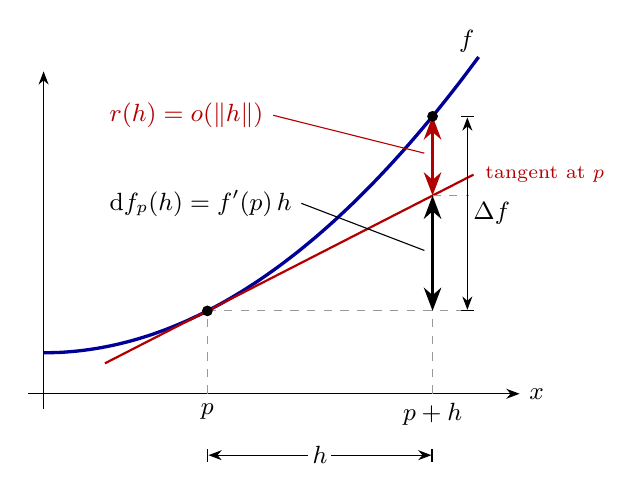
\begin{tikzpicture}[scale=1.30,>=Stealth,font=\small]
  \draw[->] (-0.15,0) -- (4.65,0) node[right]{$x$};
  \draw[->] (0,-0.15) -- (0,3.15);
  % f(x) = 0.4 + 0.16 x^2 ;  p = 1.6, p+h = 3.8
  \draw[very thick,blue!60!black,domain=0:4.25,smooth,variable=\x]
       plot ({\x},{0.4+0.16*\x*\x}) node[above left,black,inner sep=1pt]{$f$};
  % tangent at p: value 0.8096, slope 0.512
  \draw[thick,red!70!black,domain=0.60:4.20,smooth,variable=\x]
       plot ({\x},{0.8096+0.512*(\x-1.6)});
  \node[red!70!black,anchor=west,font=\scriptsize] at (4.22,2.14) {tangent at $p$};
  % helper lines
  \draw[dashed,gray!80] (1.6,0) node[below,black]{$p$} -- (1.6,0.8096);
  \draw[dashed,gray!80] (3.8,0) node[below,black]{$p+h$} -- (3.8,2.7104);
  \draw[dashed,gray!80] (1.6,0.8096) -- (4.16,0.8096);
  \draw[dashed,gray!80] (3.8,1.9360) -- (4.16,1.9360);
  % h
  \draw[|<->|] (1.6,-0.60) -- (3.8,-0.60) node[midway,fill=white,inner sep=1.5pt]{$h$};
  % Delta f on the far right
  \draw[|<->|] (4.14,0.8096) -- (4.14,2.7104)
       node[midway,right,inner sep=2pt]{$\Delta f$};
  % the two segments on the vertical at 3.8
  \draw[<->,very thick,red!70!black] (3.80,1.9360) -- (3.80,2.7104);
  \draw[<->,very thick,black]        (3.80,0.8096) -- (3.80,1.9360);
  % leader lines and labels in the empty upper-left region
  \node[anchor=west,red!70!black] (Rlab) at (0.55,2.72) {$r(h)=o(\|h\|)$};
  \draw[red!70!black,thin] (Rlab.east) -- (3.72,2.35);
  \node[anchor=west] (Dlab) at (0.55,1.86) {$\dd f_p(h)=f'(p)\,h$};
  \draw[thin] (Dlab.east) -- (3.72,1.40);
  \fill (1.6,0.8096) circle (1.5pt);
  \fill (3.8,2.7104) circle (1.5pt);
\end{tikzpicture}
\caption{Differentiability is a statement about the \emph{remainder}. The increment
$\Delta f = f(p+h)-f(p)$ splits into a piece exactly linear in the displacement --- which is
$\dd f_p$ evaluated on that displacement --- plus a remainder vanishing faster than $\|h\|$.
Note that $\dd f_p$ is defined for \emph{all} displacements $h$, not only small ones: it is a
linear map, hence determined by its values on a basis.}
\label{fig:linapprox}
\end{figure}

\section{Vectors, dual vectors, and why $\dd x^i$ is a basis}
\label{sec:dual}

\subsection{The linear algebra you already have}

Let $V$ be a real vector space of dimension $n$. Its \emph{dual}
$V^*=\{\text{linear maps }V\to\R\}$ is again $n$-dimensional, and given a basis $\{e_i\}$ of
$V$ the \emph{dual basis} $\{\varepsilon^i\}$ of $V^*$ is \emph{defined} by
\begin{equation}
\varepsilon^i(e_j)\;=\;\delta^i_{\,j}.
\label{eq:dualbasis}
\end{equation}
That one equation fixes each $\varepsilon^i$ completely, because a linear map is determined by
its values on a basis. Immediately: $\varepsilon^i$ reads off the $i$-th component of a vector,
any $\omega\in V^*$ is $\omega=\omega_i\varepsilon^i$ with $\omega_i=\omega(e_i)$, and
$\omega(\vv)=\omega_iv^i$. There is no canonical way to identify $V$ with $V^*$ --- doing so
needs an inner product (\S\ref{sec:metric}) --- which is why upper and lower indices are worth
keeping apart.

\subsection{Tangent vectors on a manifold}

On $\R^n$ one can say ``a vector at $p$ is an arrow''. On a curved space there is no ambient
room to draw the arrow in, so one uses either of two equivalent definitions:
\begin{itemize}[leftmargin=1.3em,itemsep=1pt]
\item \emph{velocity}: $\vv$ is the velocity at $t=0$ of a curve through $p$;
\item \emph{directional derivative}: $\vv$ is the operator ``rate of change along $\vv$'',
      a linear map $\vv:C^\infty(\M)\to\R$ obeying the product
      rule\footnote{Such an operator is called a \emph{derivation} at $p$. That the derivations
      at $p$ form a vector space of dimension exactly $n$ --- with basis the $n$ coordinate
      derivatives --- is the theorem that makes this definition usable; it is proved in
      \S\ref{sec:productrule}.}
      $\vv(fg)=f(p)\vv(g)+g(p)\vv(f)$.
\end{itemize}
The bridge is $\vv(f)=\frac{\dd}{\dd t}\big|_0 f(\gamma(t))$. Either way the tangent vectors at
$p$ form an $n$-dimensional space $T_p\M$, and in a chart a basis is
\begin{equation}
\Big\{\pdi{x^1}\Big|_p,\dots,\pdi{x^n}\Big|_p\Big\},
\qquad \vv = v^i\,\pdi{x^i}\Big|_p, \qquad \vv(f)=v^i\partial_if(p).
\end{equation}
Writing $\partial/\partial x^i$ for a basis \emph{vector} is jarring at first; it is just the
operator ``differentiate along the $i$-th coordinate line''.

\subsection{The cotangent space, and the two faces of $\dd x^i$}
\label{sec:twofaces}

Define $T_p^*\M:=(T_p\M)^*$, the \emph{cotangent space}; its elements are \emph{covectors}, or
\emph{$1$-forms at $p$}. Now the point of this whole note. Take Definition~\ref{def:diff} on a
manifold: for $f\in C^\infty(\M)$ the differential is the linear map
\begin{equation}
\dd f_p:T_p\M\to\R,\qquad \dd f_p(\vv):=\vv(f).
\label{eq:dfdef}
\end{equation}
This is manifestly linear in $\vv$, so $\dd f_p\in T_p^*\M$: it is the invariant content of
``the directional derivative of $f$'', with the direction left as an argument instead of
plugged in.

Now apply \eqref{eq:dfdef} in the special case where $f$ is a \emph{coordinate function} $x^i$
--- a chart is, after all, just $n$ smooth real-valued functions:
\begin{equation}
\boxed{\ \dd x^i\Big(\pdi{x^j}\Big) \;=\; \pdi{x^j}(x^i) \;=\; \pd{x^i}{x^j} \;=\; \delta^i_{\,j}\ }
\label{eq:punchline}
\end{equation}
Compare \eqref{eq:dualbasis}. \emph{The differentials of the coordinate functions are precisely
the dual basis to the coordinate vector fields.} Nothing was postulated; it fell out of the two
definitions.

\begin{keybox}
\textbf{Answer to Q2.} ``$\dd x$ is a basis covector'' and ``$\dd x$ is the differential of the
function $x$'' are the same statement, by \eqref{eq:punchline}. So
\[
\dd f \;=\; \pd{f}{X}\dd X + \pd{f}{Y}\dd Y + \pd{f}{Z}\dd Z
\]
is an \emph{identity between linear functions} on $T_p\M$. Check it by evaluating both sides on
a basis: the left side on $\partial_Y$ gives $\partial_Yf$ by \eqref{eq:dfdef}, the right side
gives $\partial_Xf\cdot0+\partial_Yf\cdot1+\partial_Zf\cdot0$. Two linear maps agreeing on a
basis are equal. No infinitesimal appears anywhere.
\end{keybox}

\noindent A \emph{$1$-form} on $\M$ is a smooth assignment $p\mapsto\omega_p\in T_p^*\M$; these
make up $\Om^1(\M)$, and in a chart $\omega=\omega_i(x)\,\dd x^i$. Note $\Om^1(\M)$ is much
bigger than the set of $\dd f$'s: not every $1$-form is the differential of a function. That
gap is \S\ref{sec:exact}, and it is where thermodynamics lives.

\subsection{How to picture a covector}
\label{sec:covectorpicture}

A vector is an arrow. A covector is \emph{not} an arrow: it is a family of parallel level
surfaces of the linear function, with a sense of increase. Evaluating $\omega(\vv)$ means
\emph{counting how many surfaces the arrow pierces}, with sign. This is the picture in
Misner--Thorne--Wheeler \cite{MTW}, and it is worth internalising, because ``integrate a
$1$-form along a curve'' will become ``count the surfaces the curve pierces''.

\begin{figure}[h]
\centering
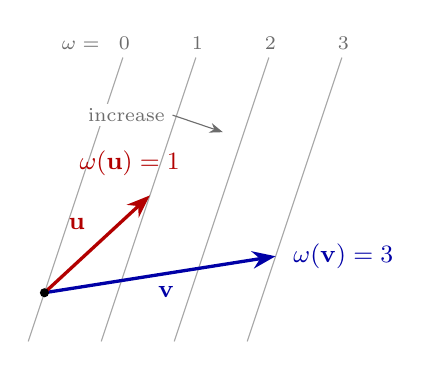
\begin{tikzpicture}[scale=1.03,>=Stealth,font=\small]
  % level sets of omega: the lines x - y/3 = 0.9k, i.e. x = 0.9k + y/3
  \foreach \k in {0,1,2,3}{
    \draw[gray!70] ({0.9*\k-0.20},-0.60) -- ({0.9*\k+0.967},2.90);
    \node[gray!85!black,font=\scriptsize,anchor=south]
        at ({0.9*\k+0.985},2.88) {$\k$};
  }
  \node[gray!85!black,font=\scriptsize,anchor=south east] at (0.80,2.88) {$\omega=$};
  % increase direction (perpendicular to the sheets, in the direction of growth)
  \draw[->,gray!85!black] (1.58,2.19) -- (2.20,1.98);
  \node[gray!85!black,font=\scriptsize,anchor=east,fill=white,inner sep=1.5pt]
      at (1.54,2.19) {increase};
  % vectors from the common origin
  \draw[->,very thick,blue!65!black] (0,0) -- (2.85,0.45);
  \node[blue!65!black,anchor=north] at (1.50,0.20) {$\vv$};
  \node[blue!65!black,anchor=west,font=\small] at (2.95,0.45) {$\omega(\vv)=3$};
  \draw[->,very thick,red!70!black] (0,0) -- (1.30,1.20);
  \node[red!70!black,anchor=south east] at (0.62,0.66) {$\uu$};
  \node[red!70!black,anchor=south,font=\small] at (1.05,1.32) {$\omega(\uu)=1$};
  \fill (0,0) circle (1.6pt);
\end{tikzpicture}
\hspace{0.55cm}
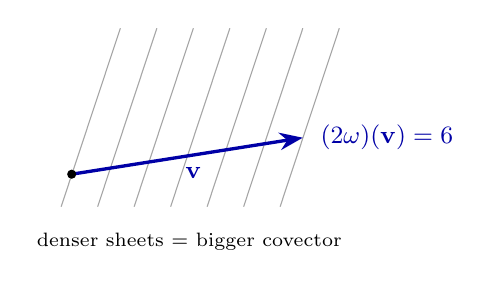
\begin{tikzpicture}[scale=1.03,>=Stealth,font=\small]
  \foreach \k in {0,1,2,3,4,5,6}{
    \draw[gray!70] ({0.45*\k-0.13},-0.40) -- ({0.45*\k+0.60},1.80);
  }
  \draw[->,very thick,blue!65!black] (0,0) -- (2.85,0.45);
  \node[blue!65!black,anchor=north] at (1.50,0.20) {$\vv$};
  \node[blue!65!black,anchor=west,font=\small] at (2.95,0.45) {$(2\omega)(\vv)=6$};
  \fill (0,0) circle (1.6pt);
  \node[font=\scriptsize,anchor=north,align=center] at (1.45,-0.60)
      {denser sheets $=$ bigger covector};
\end{tikzpicture}
\caption{A covector is not an arrow: it is a stack of parallel level surfaces
with a sense of increase, and $\omega(\vv)$ \emph{counts the surfaces pierced} by $\vv$, with
sign. Doubling $\omega$ halves the spacing (right). The dual-basis condition
$\dd x^i(\partial_j)=\delta^i_j$ says the surfaces of $\dd x^i$ are the level sets
$x^i=\text{const}$, spaced so the unit coordinate arrow $\partial_i$ pierces exactly one.}
\label{fig:covector}
\end{figure}

\subsection{Where the ``infinitesimal'' went}

The old reading ``$\dd x$ is an infinitely small displacement'' is recovered, not discarded.
Let $\vv\in T_p\M$, pick a curve $\gamma$ with $\gamma(0)=p$, $\dot\gamma(0)=\vv$, and let
$\epsilon>0$ be a small number. Then $\epsilon\vv$ is a perfectly finite tangent vector and
\begin{equation}
\dd f_p(\epsilon\vv)\;=\;\epsilon\,\dd f_p(\vv)\;=\;f(\gamma(\epsilon))-f(\gamma(0))+o(\epsilon).
\end{equation}
So $\dd f_p(\epsilon\vv)$ \emph{is} the ``infinitesimal change of $f$ under an infinitesimal
displacement'', in the only sense that survives scrutiny: it is the exact linear term. The
smallness lives in $\epsilon$, a number you control, not in $\dd$. Leibniz-notation
manipulations are legitimate because they are linear-algebra identities in disguise, and
\S\ref{sec:rules} derives them one by one.

\subsection{Gradient $\ne$ differential: a hidden metric}
\label{sec:metric}

$\dd f$ needs no extra structure. The \emph{gradient} does. If $\M$ carries a
metric\footnote{A \emph{metric} $g$ is a smooth field of inner products on the tangent spaces;
in components $\dd s^2 = g_{ij}\dd x^i\dd x^j$ is the physicist's line element.} $g$, then $g$
supplies the missing identification of $T_p\M$ with $T_p^*\M$:
\begin{equation}
\vv\mapsto\vv^\flat:=g(\vv,\cdot),\qquad \omega\mapsto\omega^\sharp,\quad
(\omega^\sharp)^i=g^{ij}\omega_j ,
\label{eq:musical}
\end{equation}
and by definition
\begin{equation}
\boxed{\ \grad f:=(\dd f)^\sharp,\qquad (\grad f)^i=g^{ij}\partial_jf .\ }
\end{equation}
In Cartesian coordinates on flat $\R^3$, $g_{ij}=\delta_{ij}$ and the components of $\grad f$
and $\dd f$ agree numerically --- which is exactly why the distinction is invisible in
elementary courses, and why curvilinear coordinates then seem to sprout mysterious factors.
In spherical coordinates, with $\dd s^2=\dd r^2+r^2\dd\theta^2+r^2\sin^2\theta\,\dd\varphi^2$,
\begin{align}
\dd f &= \pd{f}{r}\dd r+\pd{f}{\theta}\dd\theta+\pd{f}{\varphi}\dd\varphi
&&\text{(no metric; components are just partials)},\\
\grad f &= \pd{f}{r}\hat e_r+\frac1r\pd{f}{\theta}\hat e_\theta
+\frac{1}{r\sin\theta}\pd{f}{\varphi}\hat e_\varphi
&&\text{(metric used twice: }g^{ij}\text{ and unit-normalising)}.
\end{align}
The $1/r$ factors are $g^{ij}$, not magic. Check the units too: if $f$ is a temperature,
$\partial f/\partial\theta$ is K per radian, while the $\hat e_\theta$ component of $\grad f$
is K\,m$^{-1}$. \emph{The differential is the primitive object; the gradient is derived from it
using a metric.}

\begin{keybox}
\textbf{Answer to Q4b (gradient).} $\dd f$ is a covector and always exists. $\grad f$ is the
vector obtained by raising its index with the metric. On flat $\R^3$ in Cartesian coordinates
they coincide numerically and get conflated; on a curved space, in curvilinear coordinates, or
in relativity they are different objects --- and $\partial_\mu f$ versus $\partial^\mu f$ in
field theory is the same distinction.
\end{keybox}


\section{The rules of calculus, re-derived}
\label{sec:rules}

Nothing in \S\ref{sec:dual} was new content; it was a change of bookkeeping. To make that
concrete, here are the computational rules of elementary calculus, each obtained either as the
\emph{definition} of one of the objects involved or as composition of linear maps.

\subsection{The tangent map}
\label{sec:tangentmap}

One object is still missing: the derivative of a \emph{map between spaces}, as opposed to a
function. For smooth $\phi:N\to\M$ define the \emph{tangent map}
$\dd\phi_q:T_qN\to T_{\phi(q)}\M$ by
\begin{equation}
\big(\dd\phi_q\,\vv\big)(f)\;:=\;\vv\,(f\circ\phi)\qquad\text{for all }f\in C^\infty(\M).
\label{eq:pushforward}
\end{equation}
That this is well defined is one line of the product rule. In charts $u^a$ on $N$ and $x^i$ on
$\M$, taking $\vv=\partial/\partial u^a$ gives
\begin{equation}
\dd\phi_q\Big(\pdi{u^a}\Big)=\pd{\phi^i}{u^a}\pdi{x^i},
\qquad\text{i.e.}\qquad \big[\dd\phi_q\big]=\text{the Jacobian matrix.}
\label{eq:jacobianmatrix}
\end{equation}
So \emph{the Jacobian matrix is the matrix of a linear map between tangent spaces}, and when the
target is $\R$ it degenerates to the single row $\dd f$ of \eqref{eq:dfexp}.

\subsection{The product rule, and why the expansion is legitimate}
\label{sec:productrule}

\begin{keybox}
\textbf{Product rule.} For $A,B$ differentiable at $p$, $AB$ is too, and
\begin{equation}
\dd(AB)\;=\;B\,\dd A+A\,\dd B ,
\qquad\text{i.e.}\qquad
\dd(AB)_p(\vv)=B(p)\,\dd A_p(\vv)+A(p)\,\dd B_p(\vv).
\label{eq:product}
\end{equation}
\end{keybox}

\paragraph{Proof, and where the smallness is used.} Abbreviate the increments
$\Delta A:=A(p+\hh)-A(p)$ and $\Delta B$ likewise. Expanding
$(A(p)+\Delta A)(B(p)+\Delta B)$ gives an \emph{exact} identity --- no approximation anywhere:
\begin{equation}
\Delta(AB)\;=\;\underbrace{B(p)\Delta A}_{\text{1st order in }A}
+\underbrace{A(p)\Delta B}_{\text{1st order in }B}
+\underbrace{\Delta A\,\Delta B}_{\text{1st order in \emph{both}}} .
\label{eq:exactproduct}
\end{equation}
Insert $\Delta A=\dd A_p(\hh)+o(\|\hh\|)$ and the same for $B$. The first two terms give
$\big[B(p)\dd A_p+A(p)\dd B_p\big](\hh)$ plus $o(\|\hh\|)$. For the third: a linear map on a
finite-dimensional space is bounded, so $|\Delta A|=O(\|\hh\|)$ and likewise for $B$, whence
$|\Delta A\,\Delta B|=O(\|\hh\|^2)=o(\|\hh\|)$. So the remainder is $o(\|\hh\|)$ and the bracket
is linear; by the uniqueness clause of Definition~\ref{def:diff} that bracket \emph{is}
$\dd(AB)_p$. \hfill$\square$

\begin{keybox}
\textbf{Why one term may be dropped.} Identity \eqref{eq:exactproduct} is exact and has three
terms; differentiability buys exactly one thing, the licence to discard the third. $\dd A$ and
$\dd B$ are the \emph{first-order} parts of $\Delta A$ and $\Delta B$, so $\Delta A\,\Delta B$
is \emph{second} order --- and a linear map cannot contain a second-order term. The two
survivors are the two ways of being first order in one factor and zeroth in the other. This is
why the classical manipulation
$\dd(AB)=(A+\dd A)(B+\dd B)-AB\approx A\,\dd B+B\,\dd A$ is legitimate: the dropped
$\dd A\,\dd B$ is not ``too small to matter'', it is \emph{of the wrong order to belong to a
linear map at all}.
\end{keybox}

\paragraph{And why $\dd A,\dd B$ may appear on the right at all.} Equation \eqref{eq:product}
looks like a basis expansion, and $\{\dd A_p,\dd B_p\}$ is generally \emph{not} a basis of
$T_p^*\M$ --- there are $n$ of those, and these two may even be dependent or zero. But it is
not a basis expansion: it is an equality between two \emph{elements} of the vector space
$T_p^*\M$, the right-hand side being a linear combination of two covectors with the two
\emph{numbers} $B(p)$, $A(p)$ as coefficients. Three ways to see there is nothing to worry
about.

Three ways to see it. \emph{First}, the
genuine basis expansion happens earlier, in $\dd x^i$: componentwise the ordinary one-variable
product rule gives
$\dd(AB)=\partial_i(AB)\dd x^i=(B\partial_iA+A\partial_iB)\dd x^i=B\,\dd A+A\,\dd B$, so the
appearance of $\dd A$ and $\dd B$ is a \emph{regrouping of the answer}, not an expansion in
them. \emph{Second}, $AB$ depends on the point only through the two numbers $A$ and $B$, so all
a displacement can do to the product is what it does to that pair --- whence only two covectors
can appear. A check against \eqref{eq:product}: if $\vv$ lies in both $\Ker\dd A_p$ and
$\Ker\dd B_p$ then $\dd(AB)_p(\vv)=0$, i.e.\ if both factors are stationary along $\vv$ so is
the product. \emph{Third}, the degenerate cases behave: for $A,B$ constant the span is $\{0\}$;
for $B=A$, $\dd(A^2)=2A\,\dd A$ lives in a \emph{one}-dimensional span; and on $\R^5$,
$\dd(x^1x^2)=x^2\dd x^1+x^1\dd x^2$ lies in a $2$-plane, as it must, since $x^1x^2$ ignores
$x^3,x^4,x^5$.

\paragraph{Two remarks.} If you define tangent vectors as directional-derivative operators the
product rule is an \emph{axiom} and the proof is one line; the calculation above is what
justifies promoting it to one. And the axiom is not arbitrary --- it forces the coordinate
derivatives. (Sketch, $p=0$: Taylor gives $f=f(0)+x^i\partial_if(0)+x^ix^jh_{ij}$ with $h_{ij}$
smooth; such an operator kills the constant, is linear on the middle term, and annihilates the
last because \emph{both} factors of $x^i\cdot(x^jh_{ij})$ vanish at $0$ --- the same reason
$\Delta A\,\Delta B$ died above. So $\vv=\vv(x^i)\partial_i$.) Second, nothing used
commutativity or that the values were numbers, only that multiplication is linear in each factor
separately. So ``one term per slot'' is the whole rule: for matrices keep the order,
$\dd(AB)=(\dd A)B+A\,\dd B$; for inner products
$\dd\pair AB=\pair{\dd A}B+\pair A{\dd B}$; for an $n$-fold product, $n$ terms --- which is where
the $n$ in $\dd(f^n)=nf^{n-1}\dd f$ comes from; and for wedge products, one term per slot with a
sign for moving $\dd$ past a $p$-form, which is the graded rule of \S\ref{sec:extd}.

\subsection{Constants, linearity, quotient, power}

\paragraph{$\dd(\text{const})=0$.} Apply \eqref{eq:product} to $1=1\cdot1$:
$\dd(1)=2\,\dd(1)$, so $\dd(1)=0$ and $\dd c=0$. The derivative of a constant vanishing is a
\emph{consequence} of the product rule.

\paragraph{Linearity.} $\dd(af+bg)=a\,\dd f+b\,\dd g$ directly from Definition~\ref{def:diff}:
a sum of linear approximations is one.

\paragraph{Quotient and power.} From $g\cdot(1/g)=1$ and $\dd(1)=0$,
\begin{equation}
\dd\!\left(\tfrac1g\right)=-\frac{\dd g}{g^2}
\quad\Longrightarrow\quad
\dd\!\left(\frac fg\right)=\frac{g\,\dd f-f\,\dd g}{g^2},
\end{equation}
and $\dd(f^n)=nf^{n-1}\dd f$ for $n\in\Z$ by induction.

\subsection{The chain rule is the definition of the tangent map}
\label{sec:chainrule}

For $\phi:N\to\M$ and $f\in C^\infty(\M)$, read \eqref{eq:pushforward} right to left and then
use \eqref{eq:dfdef}:
\begin{equation}
\dd(f\circ\phi)_q(\vv)=\vv(f\circ\phi)=\big(\dd\phi_q\vv\big)(f)=\dd f_{\phi(q)}\big(\dd\phi_q\vv\big),
\end{equation}
that is,
\begin{equation}
\boxed{\ \dd(f\circ\phi)_q\;=\;\dd f_{\phi(q)}\circ\dd\phi_q\ }
\label{eq:chainrule}
\end{equation}
\emph{The chain rule is the definition \eqref{eq:pushforward} read backwards} --- there is
nothing to prove. In components it is matrix multiplication:
$\partial(f\circ\phi)/\partial u^a=(\partial f/\partial x^i)(\partial\phi^i/\partial u^a)$.

The same argument for two maps gives $\dd(\psi\circ\phi)=\dd\psi\circ\dd\phi$, and
$\dd(\id)=\id$; applying both to $\phi^{-1}\circ\phi=\id$,
\begin{equation}
\dd(\phi^{-1})_{\phi(p)}=\big(\dd\phi_p\big)^{-1},
\label{eq:invfn}
\end{equation}
so the Jacobian of the inverse is the inverse Jacobian --- in one dimension,
$\frac{\dd y}{\dd x}\frac{\dd x}{\dd y}=1$.

\paragraph{Why ``cancelling $\dd x$'' works, and when it does not.} Equations
\eqref{eq:chainrule} and \eqref{eq:invfn} are statements about \emph{linear maps}, and a
$1\times1$ matrix is a number: in one dimension composition is multiplication of numbers, which
commutes and can be inverted, so Leibniz notation behaves like a fraction. In two or more
dimensions $\dd\phi$ is a genuine matrix --- need not be square, need not be invertible, and
matrices do not commute. That is exactly why
$\partial f/\partial u^a=(\partial f/\partial x^i)(\partial x^i/\partial u^a)$ needs the sum
over $i$ and cannot be got by cancelling.

\paragraph{The total and material derivative.} Take $N=\R$, so $\phi=\gamma$ is a curve. Then
\eqref{eq:chainrule} reads
\begin{equation}
\frac{\dd}{\dd t}f(\gamma(t))=\dd f_{\gamma(t)}\big(\dot\gamma(t)\big)=\pd{f}{x^i}\dot x^i ,
\label{eq:totalderiv}
\end{equation}
the ``total derivative'' of multivariable calculus --- and, with $\M$ spacetime and $\gamma$ a
fluid worldline, the material derivative $Df/Dt=\partial_tf+\vv\cdot\nabla f$. Note the
right-hand side is exactly the integrand of the line integral \eqref{eq:curveint}: \emph{a line
integral is the total derivative, integrated}.

\subsection{Implicit differentiation: tangents are kernels}
\label{sec:implicit}

Let $C=\{F=c\}$ be a level set with $\dd F\ne0$ on it. A tangent vector to $C$ is the velocity
of a curve inside $C$, along which $F$ is constant, so by \eqref{eq:totalderiv}
\begin{equation}
T_pC\;=\;\Ker\dd F_p\;\subset\;T_p\R^2 .
\label{eq:tangentkernel}
\end{equation}
This is the picture of Fig.~\ref{fig:covector} read the other way: the level surfaces of the
covector $\dd F_p$ \emph{are} the level sets of $F$ to first order, and the tangent to a surface
is the kernel. Writing $\vv=a\partial_x+b\partial_y$, condition \eqref{eq:tangentkernel} is
$aF_x+bF_y=0$, so the slope of $C$ is
\begin{equation}
\frac{\dd y}{\dd x}\bigg|_C=\frac ba=-\frac{F_x}{F_y}.
\end{equation}
``Differentiate the equation and solve'' is exactly the statement that $\dd F$ vanishes on the
tangent directions. No metric was used; the familiar ``$\nabla F$ is perpendicular to the level set''
needs one, because perpendicularity does.

\subsection{Lagrange multipliers}
\label{sec:lagrange}

Extremise $f$ over the common level set of $k$ constraints,
$K=\{g^1=c^1,\dots,g^k=c^k\}$, and assume the $\dd g^a_p$ are linearly independent (so $K$ is a
surface of codimension $k$). By \eqref{eq:tangentkernel} applied $k$ times,
$T_pK=\bigcap_a\Ker\dd g^a_p$. Then $p$ is a critical point of $f$ restricted to $K$ iff $f$
changes to no first order along every admissible displacement, i.e.\ iff
\begin{equation}
\dd f_p(\vv)=0 \quad\text{for every }\vv\text{ tangent to }K .
\label{eq:annihilator}
\end{equation}
One fact of linear algebra finishes it. If $\alpha^1,\dots,\alpha^k$ are independent covectors,
the covectors vanishing on $\bigcap_a\Ker\alpha^a$ are exactly the linear combinations of the
$\alpha^a$ --- both sets have dimension $k$, and one inclusion is obvious. Hence
\begin{equation}
\boxed{\ \dd f_p\;=\;\lambda_a\,\dd g^a_p\ }
\label{eq:lagrangian}
\end{equation}

\begin{keybox}
\textbf{The multipliers are components, not auxiliaries.} \eqref{eq:lagrangian} says only that
at a constrained critical point $\dd f$ lies in the subspace of $T_p^*\M$ spanned by the
constraint differentials, and the $\lambda_a$ are its \emph{components in the basis}
$\{\dd g^a\}$ of that subspace. They exist and are unique exactly when the $\dd g^a$ are
independent --- which is the ``constraint qualification'' of optimisation theory, here visibly
a statement about a basis.
\end{keybox}

\noindent \textbf{The picture.} By \S\ref{sec:covectorpicture} a covector is a stack of level
surfaces. Condition \eqref{eq:annihilator} says: \emph{at the optimum the level surfaces of $f$
are tangent to the constraint set}. If they cut across it, moving along $K$ would pierce
surfaces and change $f$ (Fig.~\ref{fig:lagrange}).

\begin{figure}[h]
\centering
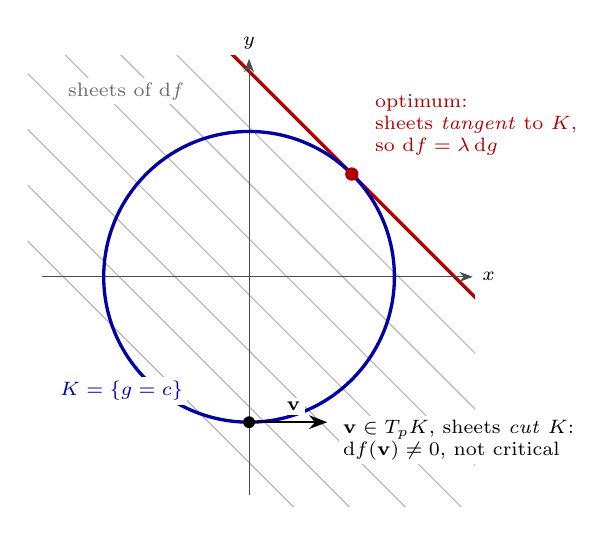
\begin{tikzpicture}[scale=1.42,>=Stealth,font=\small]
  \begin{scope}
    \clip (-1.98,-2.05) rectangle (2.02,1.98);
    % level sheets of df = dx+dy, spaced so that the tangent one is a member
    \foreach \k in {1,...,7}{
       \pgfmathsetmacro{\cc}{1.8385-0.5*\k}
       \draw[gray!58] ({\cc-2.05},2.05) -- (2.05,{\cc-2.05});
    }
    \draw[very thick,red!70!black] (-0.2115,2.05) -- (2.05,-0.2115);
  \end{scope}
  \draw[->,black!70] (-1.85,0) -- (2.00,0) node[right,black,font=\scriptsize]{$x$};
  \draw[->,black!70] (0,-1.95) -- (0,1.95) node[above,black,font=\scriptsize]{$y$};
  \draw[very thick,blue!65!black] (0,0) circle (1.3);
  \node[gray!85!black,font=\scriptsize,fill=white,inner sep=1.5pt] at (-1.10,1.66)
       {sheets of $\dd f$};
  \node[blue!65!black,font=\scriptsize,fill=white,inner sep=1.5pt] at (-1.14,-1.02)
       {$K=\{g=c\}$};
  % the optimum
  \fill[red!70!black] (0.919,0.919) circle (1.7pt);
  \node[red!70!black,anchor=south west,font=\scriptsize,align=left] at (1.04,1.00)
       {optimum:\\ sheets \emph{tangent} to $K$,\\ so $\dd f=\lambda\,\dd g$};
  % a non-critical point at the bottom of the circle
  \fill (0,-1.3) circle (1.5pt);
  \draw[->,thick] (0,-1.3) -- (0.70,-1.30);
  \node[anchor=south,font=\scriptsize,inner sep=1.5pt,fill=white] at (0.40,-1.24) {$\vv$};
  \node[anchor=west,font=\scriptsize,align=left,fill=white,inner sep=1.5pt] at (0.80,-1.46)
       {$\vv\in T_pK$, sheets \emph{cut} $K$:\\ $\dd f(\vv)\ne0$, not critical};
\end{tikzpicture}
\caption{Lagrange multipliers through the covector picture of
Fig.~\ref{fig:covector}. Grey lines are the level surfaces of $\dd f$ (here $f=x+y$), the blue
circle is the constraint set $K$. At the lower point the surfaces cut across $K$, so a
displacement $\vv$ along $K$ pierces them and $f$ can still be increased. At the optimum they
are \emph{tangent} to $K$, so $\dd f$ vanishes along $K$ --- which is \eqref{eq:lagrangian}.}
\label{fig:lagrange}
\end{figure}

\noindent\textbf{Eliminating the multipliers.} A covector lies in the span of independent
covectors iff wedging with all of them gives zero (\S\ref{sec:grassmann}), so
\eqref{eq:lagrangian} is equivalent to
\begin{equation}
\boxed{\ \dd f\wedge\dd g^1\wedge\cdots\wedge\dd g^k=0\ }
\label{eq:lagrangewedge}
\end{equation}
which never introduces the $\lambda_a$ at all.

\begin{ex}
Extremise $f=x+y$ on $g=x^2+y^2=r^2$. Then $\dd f\wedge\dd g=(\dd x+\dd y)\wedge(2x\dd x+2y\dd y)
=2(y-x)\dd x\wedge\dd y$, so \eqref{eq:lagrangewedge} gives $y=x$ immediately and
$(x,y)=\pm(r/\sqrt2,r/\sqrt2)$ --- the tangency of Fig.~\ref{fig:lagrange}. If you want the
multiplier, read it off from \eqref{eq:lagrangian}: $\lambda=1/2x$.
\end{ex}

\noindent\textbf{What the multiplier means.} Let $p(c)$ be the optimum as a function of the
constraint \emph{levels}. Differentiating $f(p(c))$ and using \eqref{eq:lagrangian} with
$g^a(p(c))=c^a$ gives
\begin{equation}
\pd{}{c^a}f\big(p(c)\big)=\lambda_a :
\label{eq:envelope}
\end{equation}
\emph{the multiplier is the sensitivity of the optimal value to relaxing its constraint} --- the
``shadow price'', and the reason the multipliers of thermodynamics turn out to be $1/T$, $p/T$,
$-\mu/T$ (\S\ref{sec:minim}).

\subsection{The thermodynamic triple product rule}
\label{sec:triple}

A rule that reliably confuses: for three quantities constrained by one equation,
\begin{equation}
\left(\pd{x}{y}\right)_{\!z}\left(\pd{y}{z}\right)_{\!x}\left(\pd{z}{x}\right)_{\!y}=-1 .
\label{eq:triple}
\end{equation}
Why $-1$? Let $f(x,y,z)=0$ define a surface $\Sigma\subset\R^3$. On $\Sigma$ the three covectors
$\dd x,\dd y,\dd z$ live in a \emph{two}-dimensional cotangent space, so they satisfy exactly
one relation, namely $\dd f=0$:
\begin{equation}
f_x\,\dd x+f_y\,\dd y+f_z\,\dd z=0\qquad\text{on }\Sigma .
\label{eq:onerelation}
\end{equation}
The notation $(\partial x/\partial y)_z$ means: move along the curve on which $z$ is constant,
i.e.\ impose $\dd z=0$. Then \eqref{eq:onerelation} collapses to $f_x\dd x+f_y\dd y=0$, whence
\begin{equation}
\left(\pd{x}{y}\right)_{\!z}=-\frac{f_y}{f_x},\qquad
\left(\pd{y}{z}\right)_{\!x}=-\frac{f_z}{f_y},\qquad
\left(\pd{z}{x}\right)_{\!y}=-\frac{f_x}{f_z},
\end{equation}
and the product is $(-1)^3$. The minus sign is a parity count, nothing more. Reading the same
ratio both ways gives the reciprocal rule $(\partial x/\partial y)_z=1/(\partial y/\partial x)_z$.

\subsection{Substitution and integration by parts}

For completeness, the two remaining rules of one-variable calculus are theorems about
\emph{integration}, and each is one line once \S\ref{sec:integration}--\S\ref{sec:stokes} are in
place. \emph{Substitution} is the statement that integration does not care whether you change
variables before or after: $\int_{\phi\circ c}\omega=\int_c\phi^*\omega$, which on $\R$ with
$\omega=f\,\dd x$ and $\phi^*\dd x=\phi'(u)\dd u$ is
$\int f(x)\dd x=\int f(\phi(u))\phi'(u)\dd u$. The ``$\dd x=\phi'(u)\dd u$'' written in every
margin is literally the pullback of a $1$-form, \eqref{eq:pullbackcoord}.
\emph{Integration by parts} is Stokes applied to $\dd(fg)=f\dd g+g\dd f$ over a curve $c$:
\begin{equation}
\int_c f\,\dd g=\int_{\partial c}fg-\int_c g\,\dd f ,
\label{eq:ibp}
\end{equation}
which on $c=[a,b]$ is $\int_a^b fg'\dd x=[fg]_a^b-\int_a^b f'g\,\dd x$.

\section{Higher derivatives: three different objects}
\label{sec:higher}

``The second derivative'' resolves into three inequivalent notions, and mixing them up is a
standard source of confusion.

\paragraph{(i) The Hessian is a bilinear form, and it is not a tensor.} Iterating
Definition~\ref{def:diff} on $p\mapsto\dd f_p$ gives, in a chart, the array
$\partial_i\partial_jf$. Under a change of coordinates it transforms as
\begin{equation}
\pd{^2f}{x'^i\partial x'^j}=\pd{x^k}{x'^i}\pd{x^l}{x'^j}\partial_k\partial_lf
+\underbrace{\pd{^2x^k}{x'^i\partial x'^j}\,\partial_kf}_{\text{inhomogeneous!}} ,
\label{eq:hesstransf}
\end{equation}
and the second term spoils tensoriality. There are exactly two standard repairs. At a
\emph{critical point} ($\dd f_p=0$) the offending term dies, so the Hessian at a critical point
\emph{is} a well-defined symmetric bilinear form on $T_p\M$ --- which is why stability analysis
of equilibria is coordinate-independent (\S\ref{sec:minim}). Alternatively, with a
connection\footnote{A \emph{connection} is the extra structure that lets you compare vectors at
different points --- covariant differentiation. Its Christoffel symbols $\Gamma^k_{ij}$ are
exactly what is needed to cancel the inhomogeneous term.} $\nabla$, set
$\nabla_i\nabla_jf=\partial_i\partial_jf-\Gamma^k_{ij}\partial_kf$, a genuine symmetric tensor.

\paragraph{(ii) $\dd\dd f=0$ is \emph{not} the second derivative.} The exterior derivative
(\S\ref{sec:extd}) applied twice gives zero:
\begin{equation}
\dd(\dd f)=\dd\big(\partial_if\,\dd x^i\big)=\partial_j\partial_if\;\dd x^j\wedge\dd x^i=0 ,
\label{eq:ddzero}
\end{equation}
because $\partial_j\partial_if$ is symmetric in $ij$ while $\dd x^j\wedge\dd x^i$ is
antisymmetric. So $\dd^2=0$ does not say second derivatives vanish; it says the exterior
derivative sees only the \emph{antisymmetric} part of $\partial\partial$, which is zero for a
function. Identity \eqref{eq:ddzero} is the source of $\curl\grad=0$, of $\dive\curl=0$, and of
the homogeneous Maxwell equations.

\paragraph{(iii) Taylor data.} The full local second-order information is the symmetric array
of Taylor coefficients,
\begin{equation}
f(p+\hh)=f(p)+\dd f_p(\hh)+\tfrac12(\partial_i\partial_jf)(p)h^ih^j+o(\|\hh\|^2),
\end{equation}
which is not a tensor (by (i)) and is symmetric (hence invisible to (ii)). \emph{Forms are the
calculus of first derivatives} --- and that is a feature, because it is first derivatives that
Stokes' theorem relates to boundaries.

\begin{keybox}
\textbf{Answer to Q4c (higher derivatives).} $\dd$ maps $\Om^p\to\Om^{p+1}$ and iterating gives
zero, so it does not generate higher derivatives. Higher derivatives of a function are
(a) non-tensorial unless you add a connection, and (b) symmetric, hence invisible to the
antisymmetric machinery of forms.
\end{keybox}


\section{Wedge products and the exterior derivative}
\label{sec:grassmann}

\subsection{Why products of differentials antisymmetrise}

Let $\Lambda^p(V^*)$ be the space of \emph{alternating} $p$-linear maps
$V\times\cdots\times V\to\R$: linear in each slot, and changing sign when two arguments are
swapped. Set $\Lambda^0=\R$ and $\Lambda^1(V^*)=V^*$. The \emph{wedge
product}\footnote{Also called the exterior product; the algebra it generates is the
\emph{Grassmann algebra}, Hassani ch.\ 3.} is the antisymmetrised tensor product; for $1$-forms
we take
\begin{equation}
(\alpha\wedge\beta)(\uu,\vv)=\alpha(\uu)\beta(\vv)-\alpha(\vv)\beta(\uu),
\quad
(\alpha^1\wedge\cdots\wedge\alpha^p)(\vv_1,\dots,\vv_p)=\det\!\big[\alpha^i(\vv_j)\big].
\label{eq:wedgedet}
\end{equation}
It is associative, and $\alpha\wedge\beta=(-1)^{pq}\beta\wedge\alpha$; in particular
$\alpha\wedge\alpha=0$ for a $1$-form. If $\{\varepsilon^i\}$ is a basis of $V^*$ then the
products $\varepsilon^{i_1}\wedge\cdots\wedge\varepsilon^{i_p}$ with $i_1<\cdots<i_p$ are a
basis of $\Lambda^p(V^*)$, so $\dim\Lambda^p=\binom np$ and $\Lambda^p=0$ for $p>n$. Doing all
of this at each point of $\M$ gives the \emph{differential $p$-forms} $\Om^p(\M)$: in a chart,
$\omega=\frac{1}{p!}\omega_{i_1\cdots i_p}(x)\,\dd x^{i_1}\wedge\cdots\wedge\dd x^{i_p}$ with
totally antisymmetric components.

\begin{keybox}
\textbf{What a $p$-form is, operationally.} It is a machine that eats $p$ tangent vectors and
returns a number, linearly in each and antisymmetrically overall. By \eqref{eq:wedgedet} that
number is a \emph{determinant}, and a determinant of $p$ vectors is the \emph{signed
$p$-volume} of the box they span. Hence \emph{a $p$-form measures oriented $p$-dimensional
volume} --- which is the entire reason forms are the integrands of $p$-dimensional integrals.
\end{keybox}

\noindent Concretely on $\R^2$, with $\uu=u^1\partial_x+u^2\partial_y$ and similarly $\vv$,
\begin{equation}
(\dd x\wedge\dd y)(\uu,\vv)=u^1v^2-v^1u^2
=\det\begin{pmatrix}u^1&v^1\\u^2&v^2\end{pmatrix},
\label{eq:areaform}
\end{equation}
the signed area of the parallelogram on $\uu,\vv$. Swap the vectors and the sign flips:
antisymmetry \emph{is} orientation. This is why $\dd x\,\dd y$ in a double integral secretly
means $\dd x\wedge\dd y$, and why $\dd x\wedge\dd x=0$ --- a degenerate parallelogram has no
area.

\begin{figure}[h]
\centering
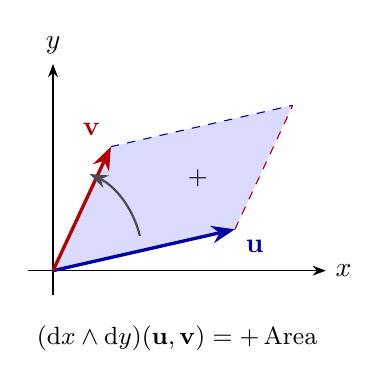
\begin{tikzpicture}[scale=1.05,>=Stealth]
  \draw[->] (-0.3,0) -- (3.3,0) node[right]{$x$};
  \draw[->] (0,-0.3) -- (0,2.5) node[above]{$y$};
  \fill[blue!14] (0,0) -- (2.2,0.5) -- (2.9,2.0) -- (0.7,1.5) -- cycle;
  \draw[->,very thick,blue!65!black] (0,0) -- (2.2,0.5) node[below right]{$\uu$};
  \draw[->,very thick,red!70!black]  (0,0) -- (0.7,1.5) node[above left]{$\vv$};
  \draw[blue!65!black,dashed] (0.7,1.5) -- (2.9,2.0);
  \draw[red!70!black,dashed]  (2.2,0.5) -- (2.9,2.0);
  % orientation arc
  \draw[->,thick,black!70] (1.05,0.42) arc (13:65:1.1);
  \node[font=\small] at (1.75,1.12) {$+$};
  \node[font=\small,anchor=north,align=center] at (1.5,-0.55)
    {$(\dd x\wedge \dd y)(\uu,\vv) = +\,\mathrm{Area}$};
\end{tikzpicture}
\hspace{0.6cm}
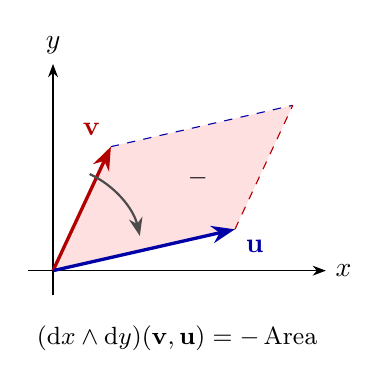
\begin{tikzpicture}[scale=1.05,>=Stealth]
  \draw[->] (-0.3,0) -- (3.3,0) node[right]{$x$};
  \draw[->] (0,-0.3) -- (0,2.5) node[above]{$y$};
  \fill[red!12] (0,0) -- (2.2,0.5) -- (2.9,2.0) -- (0.7,1.5) -- cycle;
  \draw[->,very thick,red!70!black]  (0,0) -- (0.7,1.5) node[above left]{$\vv$};
  \draw[->,very thick,blue!65!black] (0,0) -- (2.2,0.5) node[below right]{$\uu$};
  \draw[blue!65!black,dashed] (0.7,1.5) -- (2.9,2.0);
  \draw[red!70!black,dashed]  (2.2,0.5) -- (2.9,2.0);
  \draw[<-,thick,black!70] (1.05,0.42) arc (13:65:1.1);
  \node[font=\small] at (1.75,1.12) {$-$};
  \node[font=\small,anchor=north,align=center] at (1.5,-0.55)
    {$(\dd x\wedge \dd y)(\vv,\uu) = -\,\mathrm{Area}$};
\end{tikzpicture}
\caption{The 2-form $\dd x \wedge \dd y$ evaluated on two tangent vectors returns the signed
area of the parallelogram they span, \eqref{eq:areaform}. The sign is the orientation.
A 2-form is a field of such area-meters; a $p$-form is a field of oriented
$p$-volume-meters. This is the object that belongs under a $p$-dimensional integral sign.}
\label{fig:wedge}
\end{figure}

\subsection{The Jacobian is not an extra rule --- it is $\wedge$}
\label{sec:pullback}

Let $\phi:N\to\M$ be smooth. The \emph{pullback}\footnote{Forms pull \emph{back}, against the
direction of the map, whereas vectors push forward. That is the practical advantage of
covariant objects: you never need $\phi$ to be invertible to pull back a form.}
$\phi^*:\Om^p(\M)\to\Om^p(N)$ feeds the machine the pushed-forward vectors,
$(\phi^*\omega)(\vv_1,\dots,\vv_p):=\omega(\dd\phi\,\vv_1,\dots,\dd\phi\,\vv_p)$. It commutes
with everything: $\phi^*(\alpha\wedge\beta)=\phi^*\alpha\wedge\phi^*\beta$,
$\phi^*(\dd\omega)=\dd(\phi^*\omega)$, and on functions $\phi^*f=f\circ\phi$. On coordinate
differentials it is just the chain rule,
\begin{equation}
\phi^*(\dd x^i)=\dd(x^i\circ\phi)=\pd{\phi^i}{u^a}\,\dd u^a .
\label{eq:pullbackcoord}
\end{equation}
Now pull back a top-degree form on an $n$-dimensional space. Using \eqref{eq:pullbackcoord} and
\eqref{eq:wedgedet},
\begin{equation}
\boxed{\ \phi^*\!\big(f\,\dd x^1\wedge\cdots\wedge\dd x^n\big)
=(f\circ\phi)\,\det\!\left(\pd{\phi^i}{u^a}\right)\dd u^1\wedge\cdots\wedge\dd u^n .\ }
\label{eq:changeofvar}
\end{equation}
The determinant appeared \emph{by itself}, out of antisymmetry. Equation \eqref{eq:changeofvar}
is the change-of-variables formula, which in the traditional presentation must be proved as a
theorem about measures with a mysterious $|\det J|$ inserted by hand. Note also that
\eqref{eq:changeofvar} carries $\det J$ with its \emph{sign}, not $|\det J|$: forms know about
orientation, measures do not (\S\ref{sec:volume}).

\begin{ex}[Polar coordinates]\label{ex:polar}
$\phi(r,\theta)=(r\cos\theta,r\sin\theta)$, so $\phi^*\dd x=\cos\theta\,\dd r-r\sin\theta\,\dd\theta$
and $\phi^*\dd y=\sin\theta\,\dd r+r\cos\theta\,\dd\theta$. Wedging, and using
$\dd r\wedge\dd r=\dd\theta\wedge\dd\theta=0$ and $\dd\theta\wedge\dd r=-\dd r\wedge\dd\theta$,
\begin{equation}
\phi^*(\dd x\wedge\dd y)=r\cos^2\theta\;\dd r\wedge\dd\theta-r\sin^2\theta\;\dd\theta\wedge\dd r
=r\,\dd r\wedge\dd\theta .
\end{equation}
The famous factor $r$ is the Jacobian, produced by two lines of algebra.
\end{ex}

\begin{keybox}
\textbf{Answer to Q7a.} $\int\dd x\,\dd y\,f$ means $\int_S f\,\dd x\wedge\dd y$: the integral
of a $2$-form over an oriented two-dimensional domain. The juxtaposition ``$\dd x\,\dd y$''
\emph{is} the wedge product; the classical notation hides it, which is why the classical
formalism needs a separate theorem to supply the Jacobian.
\end{keybox}

\subsection{One derivative operator}
\label{sec:extd}

\begin{defn}\label{def:extd}
The \emph{exterior derivative} is the unique family of linear maps
$\dd:\Om^p(\M)\to\Om^{p+1}(\M)$ with (i) on functions it is the differential
\eqref{eq:dfdef}; (ii) $\dd(\alpha\wedge\beta)=\dd\alpha\wedge\beta+(-1)^p\alpha\wedge\dd\beta$
for $\alpha\in\Om^p$; (iii) $\dd\circ\dd=0$. In coordinates,
\begin{equation}
\dd\big(\omega_{i_1\cdots i_p}\dd x^{i_1}\wedge\cdots\wedge\dd x^{i_p}\big)
=\pd{\omega_{i_1\cdots i_p}}{x^j}\,\dd x^j\wedge\dd x^{i_1}\wedge\cdots\wedge\dd x^{i_p} .
\end{equation}
\end{defn}
\noindent Rule (ii) is the product rule of \S\ref{sec:productrule} --- one term per factor ---
with a sign for moving $\dd$ past a $p$-form. Crucially, $\dd$ needs \emph{no} metric, \emph{no}
connection, and commutes with pullback; it is the only natural first-order operator with those
properties, which is why it is the one that appears in Stokes' theorem and in gauge theory.

\subsection{$\grad$, $\curl$, $\dive$ are one operator in disguise}

On $\R^3$ with the Euclidean metric and an orientation we have two extra structures: the
raising/lowering of \S\ref{sec:metric}, and the \emph{Hodge star}\footnote{$\star$ turns a
$p$-form into an $(n-p)$-form by ``taking the orthogonal complement'', and needs a metric
\emph{and} an orientation. On $\R^3$: $\star\dd x=\dd y\wedge\dd z$,
$\star(\dd y\wedge\dd z)=\dd x$, $\star1=\dd x\wedge\dd y\wedge\dd z$, and cyclic.} $\star$.
With these, all of vector calculus is the single ladder
$\Om^0\to\Om^1\to\Om^2\to\Om^3$ read through Fig.~\ref{fig:ladder}: explicitly, with
$\A=A_i\dd x^i$,
\begin{align}
\dd f &= \partial_if\,\dd x^i && \longleftrightarrow && \grad f,\\
\dd(A_i\dd x^i) &= (\partial_1A_2-\partial_2A_1)\dd x^1\wedge\dd x^2+\text{cyc.}
  && \longleftrightarrow && \curl\A,\\
\dd\big(\star(A_i\dd x^i)\big) &= (\partial_iA^i)\,\dd x^1\wedge\dd x^2\wedge\dd x^3
  && \longleftrightarrow && \dive\A .
\end{align}
The Laplacian is $\Delta f=\star\,\dd\star\dd f$, and the general second-order operator is
$\Delta=\dd\,\dd^\dagger+\dd^\dagger\dd$ with $\dd^\dagger=\pm\star\dd\star$ the
\emph{codifferential} --- the formal adjoint of $\dd$ (\S\ref{sec:adjoint}).

\begin{figure}[h]
\centering
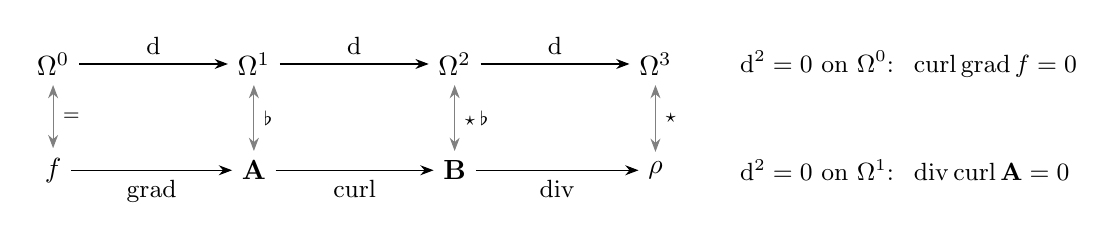
\begin{tikzpicture}[>=Stealth,node distance=2.55cm]
  \node (O0) {$\Om^0$};
  \node (O1) [right of=O0] {$\Om^1$};
  \node (O2) [right of=O1] {$\Om^2$};
  \node (O3) [right of=O2] {$\Om^3$};
  \draw[->] (O0) -- node[above,font=\small]{$\dd$} (O1);
  \draw[->] (O1) -- node[above,font=\small]{$\dd$} (O2);
  \draw[->] (O2) -- node[above,font=\small]{$\dd$} (O3);
  \node (F0) [below of=O0,node distance=1.35cm] {$f$};
  \node (F1) [below of=O1,node distance=1.35cm] {$\A$};
  \node (F2) [below of=O2,node distance=1.35cm] {$\B$};
  \node (F3) [below of=O3,node distance=1.35cm] {$\rho$};
  \draw[->] (F0) -- node[below,font=\small]{$\grad$} (F1);
  \draw[->] (F1) -- node[below,font=\small]{$\curl$} (F2);
  \draw[->] (F2) -- node[below,font=\small]{$\dive$} (F3);
  \draw[<->,gray] (O0) -- node[right,font=\scriptsize,black]{$=$} (F0);
  \draw[<->,gray] (O1) -- node[right,font=\scriptsize,black]{$\flat$} (F1);
  \draw[<->,gray] (O2) -- node[right,font=\scriptsize,black]{$\star\,\flat$} (F2);
  \draw[<->,gray] (O3) -- node[right,font=\scriptsize,black]{$\star$} (F3);
  \node[anchor=west,align=left,font=\small] at (8.6,0.0)
     {$\dd^2=0$ on $\Om^0$: $\ \curl\grad f = 0$};
  \node[anchor=west,align=left,font=\small] at (8.6,-1.35)
     {$\dd^2=0$ on $\Om^1$: $\ \dive\curl\A = 0$};
\end{tikzpicture}
\caption{Vector calculus on $\R^3$ as one operator. The vertical maps use the
metric and the orientation; the horizontal ones use neither. All three of $\grad$, $\curl$,
$\dive$ are $\dd$ acting in different degrees, and the two classical vanishing identities are
the single statement $\dd^2=0$. In $n\ne3$ dimensions the ladder is longer or shorter and there
is no ``curl'' --- the vector-calculus packaging is an accident of three dimensions.}
\label{fig:ladder}
\end{figure}

\begin{keybox}
\textbf{Answer to Q4d (curl).} $\curl$ is $\dd:\Om^1\to\Om^2$, dressed with index-lowering on
the way in and $\star$ on the way out. It looks like a vector only because in three dimensions
$\binom32=3=\binom31$. In four dimensions the ``curl'' of a $1$-form is a $2$-form with
$\binom42=6$ components --- which is exactly the electromagnetic field tensor $F_{\mu\nu}$
(\S\ref{sec:de}).
\end{keybox}


\section{Integration as a pairing between domains and forms}
\label{sec:integration}

\subsection{First question: what \emph{kind} of object can be integrated?}

Before asking what $\int$ means, ask what it can eat. To integrate ``something'' along a curve
you must parametrise, $\gamma:[0,1]\to\M$; the answer must not depend on the parametrisation,
or it is not a property of the curve.

Try a \emph{function} $f$. The only candidate is $\int_0^1 f(\gamma(t))\dd t$. Reparametrise by
$t=h(s)$ with $h$ increasing, $h(0)=0$, $h(1)=1$: with $\M=\R$, $\gamma(t)=t$, $f(x)=x$ and
$h(s)=s^2$ the two integrals are $\tfrac12$ and $\tfrac13$. \emph{Functions cannot be integrated
over curves.} To rescue this you must supply extra structure --- an arclength element
$\dd s=\sqrt{g_{ij}\dot x^i\dot x^j}\,\dd t$, which needs a metric.

Now try a $1$-form $\omega$. The only candidate is
\begin{equation}
\int_\gamma\omega:=\int_0^1\omega_{\gamma(t)}\big(\dot\gamma(t)\big)\dd t ,
\label{eq:curveint}
\end{equation}
where $\dot\gamma(t)\in T_{\gamma(t)}\M$ is the velocity. Reparametrising sends
$\dot\gamma\to\dot\gamma\,h'(s)$, and $\omega$ is \emph{linear} in its argument, so the
integrand picks up exactly the factor $h'(s)$ that $\dd t=h'(s)\dd s$ needs, and the answer is
unchanged. It works, and it works because of linearity in the tangent vector. The same
computation in $p$ dimensions works because a $p$-form is multilinear and alternating, so it
absorbs precisely the Jacobian determinant of a reparametrisation, \eqref{eq:changeofvar}.

\begin{keybox}
\textbf{Why forms.} $p$-forms are not a fancy repackaging of integrands; they are \emph{the
only kind of object that can be integrated over an oriented $p$-dimensional domain without
extra structure}, because their transformation law under reparametrisation is exactly inverse to
that of the parameter volume element. ``$f\,\dd x$'' was always a $1$-form; the classical
notation simply did not name it.
\end{keybox}

\subsection{The definition, in general}

\begin{defn}[Domains and integration]\label{def:int}
A \emph{$p$-cube} in $\M$ is a smooth map $c:[0,1]^p\to\M$, and a \emph{$p$-chain}\footnote{The
coefficients let you glue pieces and reverse orientations: $-c$ means $c$ traversed backwards.
``Chain'' is just a bookkeeping word for a signed collection of parametrised patches.} is a
finite formal sum $c=\sum_ka_kc_k$. The \emph{boundary} $\partial c$ is the signed sum of the
faces, with signs arranged so that $\partial\partial=0$. For $\omega\in\Om^p(\M)$ and a
$p$-cube $c$, pull back to the parameter cube: $c^*\omega$ is a $p$-form on $[0,1]^p$, hence of
the form $g(u)\,\dd u^1\wedge\cdots\wedge\dd u^p$ for a \emph{single} function $g$, since
$\Lambda^p$ of a $p$-dimensional space is one-dimensional. Define
\begin{equation}
\boxed{\ \int_c\omega\;:=\;\int_{[0,1]^p}g(u)\,\dd u^1\cdots\dd u^p\ }
\label{eq:defint}
\end{equation}
with the right-hand side an ordinary Riemann integral, and extend to chains by linearity.
\end{defn}

\noindent Two remarks. It is well defined: by \eqref{eq:changeofvar} a change of parameters
multiplies $g$ by $\det J$ and the measure by $|\det J|$, and these agree when the
reparametrisation preserves orientation. And it \emph{does} reduce to ordinary calculus --- the
right-hand side of \eqref{eq:defint} is the only place a genuine limit of sums occurs;
everything above it is linear algebra.

\subsection{The Riemann sum, re-read}

Take $\M=\R$, $c=[a,b]$, $\omega=f\,\dd x$; then \eqref{eq:defint} returns the familiar
$\int_a^bf(x)\dd x$. But look at the Riemann sum through the new lens. Partition into
sub-intervals and let $\Delta_k:=(x_{k+1}-x_k)\,\partial_x\in T_{x_k}\R$ be the \emph{tangent
vector} of the $k$-th piece. Then
\begin{equation}
\sum_kf(x_k)\,\Delta x_k=\sum_k\big(f\,\dd x\big)_{x_k}\!\big(\Delta_k\big)
\xrightarrow[N\to\infty]{}\int_{[a,b]}f\,\dd x .
\label{eq:riemannsum}
\end{equation}
The Riemann sum is: \emph{chop the domain into small oriented pieces, hand each piece's tangent
vector to the form, add up the numbers}. The form is the measuring device, the domain supplies
the things to be measured, and the integral is the total reading. In $p$ dimensions, replace
``tangent vector'' by ``the $p$ edge vectors of a small box'', which the $p$-form turns into a
signed volume.

\begin{figure}[h]
\centering
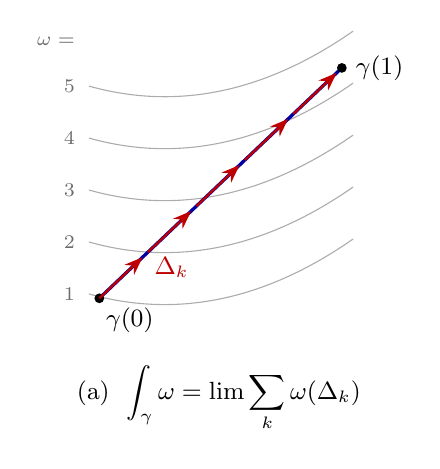
\begin{tikzpicture}[scale=1.10,>=Stealth]
  \foreach \k in {1,2,3,4,5}{
    \draw[gray!65] plot[smooth,domain=0:3.05,variable=\x]
        ({\x},{0.60*\k - 0.34 + 0.16*\x*\x - 0.28*\x});
    \node[gray!85!black,font=\scriptsize,anchor=east] at (-0.05,{0.60*\k-0.34}) {$\k$};
  }
  \node[gray!85!black,font=\scriptsize,anchor=east] at (-0.05,3.18) {$\omega=$};
  \draw[very thick,blue!65!black] (0.12,0.21) -- (2.92,2.87);
  \fill (0.12,0.21) circle (1.6pt);
  \node[font=\small,anchor=north west,inner sep=1pt] at (0.16,0.14) {$\gamma(0)$};
  \fill (2.92,2.87) circle (1.6pt);
  \node[font=\small,anchor=west,inner sep=3pt] at (2.98,2.87) {$\gamma(1)$};
  \foreach \s in {0.12,0.68,1.24,1.80,2.36}{
     \draw[->,red!75!black,thick]
        ({\s},{0.21+0.95*(\s-0.12)}) -- ({\s+0.50},{0.21+0.95*(\s+0.50-0.12)});
  }
  \node[red!75!black,font=\small,anchor=north west,inner sep=1pt] at (0.72,0.72) {$\Delta_k$};
  \node[font=\small,anchor=north] at (1.5,-0.45)
     {(a)\ \ $\displaystyle\int_\gamma\omega=\lim\sum_k \omega(\Delta_k)$};
\end{tikzpicture}
\hspace{0.85cm}
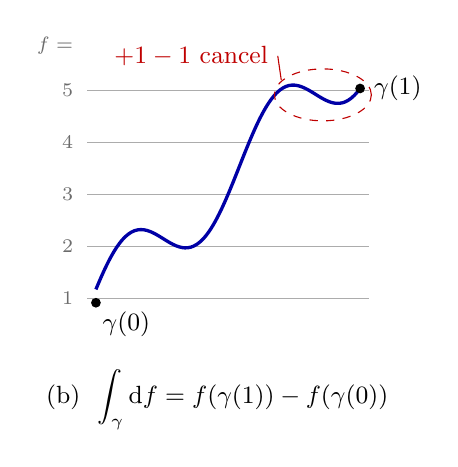
\begin{tikzpicture}[scale=1.10,>=Stealth]
  \foreach \k in {1,2,3,4,5}{
    \draw[gray!65] (0,{0.60*\k-0.34}) -- (3.25,{0.60*\k-0.34});
    \node[gray!85!black,font=\scriptsize,anchor=east] at (-0.05,{0.60*\k-0.34}) {$\k$};
  }
  \node[gray!85!black,font=\scriptsize,anchor=east] at (-0.05,3.18) {$f=$};
  \draw[very thick,blue!65!black] plot[smooth,domain=0.10:3.15,samples=90,variable=\x]
       ({\x},{0.21+0.95*(\x-0.10)+0.44*sin(\x*205)});
  \fill (0.10,0.21) circle (1.6pt);
  \node[font=\small,anchor=north west,inner sep=1pt] at (0.14,0.14) {$\gamma(0)$};
  \fill (3.15,2.684) circle (1.6pt);
  \node[font=\small,anchor=west,inner sep=3pt] at (3.21,2.684) {$\gamma(1)$};
  % ring the detour where the sheet f=5 is crossed three times
  \draw[dashed,red!75!black] (2.72,2.61) ellipse (0.56 and 0.30);
  \node[red!75!black,font=\small,anchor=west] (Nlab) at (0.20,3.06) {$+1-1$ cancel};
  \draw[red!75!black,thin] (Nlab.east) -- (2.24,2.78);
  \node[font=\small,anchor=north] at (1.5,-0.45)
     {(b)\ \ $\displaystyle\int_\gamma \dd f = f(\gamma(1))-f(\gamma(0))$};
\end{tikzpicture}
\caption{(a) Integrating a $1$-form along a curve: chop the curve, hand each
little tangent vector $\Delta_k$ to the form, add the numbers --- equivalently, count the level
surfaces of $\omega$ that $\gamma$ pierces. (b) If $\omega=\dd f$ those surfaces are the level
sets of $f$, so wherever the curve doubles back a pair of contributions cancels (dashed ring)
and only the endpoint values survive. This is the fundamental theorem of calculus, seen.}
\label{fig:riemann}
\end{figure}

\subsection{The answer to the ``finite integral'' question}

Here is the misconception worth naming. One is tempted to read $\int_a^b\dd x\,f(x)$ as ``a
linear transformation applied to the cotangent-space element $\dd x$''. It is not, and it cannot
be: $\dd x|_x$ lives in a \emph{different} one-dimensional vector space $T_x^*\R$ for each point
$x\in[a,b]$, and no linear map could take an $[a,b]$-worth of them to a number in a
coordinate-independent way. The correct statement is one level up.

\begin{keybox}
\textbf{Answer to Q6.} Integration is a \emph{bilinear pairing between a domain and an
integrand}:
\begin{equation}
\pair{\cdot}{\cdot}: \{p\text{-chains}\}\times\Om^p(\M)\to\R,
\qquad \pair{c}{\omega}:=\int_c\omega .
\label{eq:pairing}
\end{equation}
Fix $c$ and vary $\omega$: you get a linear function on the infinite-dimensional space of
$p$-\emph{forms} --- \emph{this} is the sense in which ``$\int_a^b$'' belongs to a dual space,
namely the dual of the space of forms, not the dual of a tangent space. Linearity here is the
elementary $\int(\alpha\omega_1+\beta\omega_2)=\alpha\int\omega_1+\beta\int\omega_2$. Fix
$\omega$ and vary $c$: you get additivity over subdivision, $\int_{c_1+c_2}=\int_{c_1}+\int_{c_2}$,
and orientation reversal, $\int_b^a=-\int_a^b$. The $\dd x$ inside the integral sign is the
pointwise object and enters only through Definition~\ref{def:int}.
\end{keybox}

\noindent The two operators $\partial$ (on domains) and $\dd$ (on forms) are \emph{adjoint} with
respect to \eqref{eq:pairing}; that statement is Stokes' theorem, \S\ref{sec:stokes}.

\begin{rmk}[Why the orientation sign is natural]
Elementary calculus has the awkward convention $\int_b^a=-\int_a^b$, which sits badly with the
idea of an integral as an area. In the language of forms there is nothing to reconcile: $-c$ is
a genuinely different domain from $c$, and the pairing is linear, so the sign is forced.
Unsigned integration is the \emph{other} construction, over densities rather than forms.
\end{rmk}

\subsection{Multiple integrals, volume forms, and $\sqrt{g}$}
\label{sec:volume}

For $p=n$, $\Om^n(\M)$ is one-dimensional at each point, so a top form is ``$f$ times a
reference volume form''. Three objects are worth keeping apart.

\paragraph{The coordinate volume form.} $\dd x^1\wedge\cdots\wedge\dd x^n$ is a volume form in a
chart but is chart-\emph{dependent}: by \eqref{eq:changeofvar} it acquires $\det J$. So
``$\int\dd^3x\,f$'' is meaningful only once you say which chart, or once $f$ is understood to
transform compensatingly.

\paragraph{The metric volume form.} Given a metric and an orientation,
\begin{equation}
\vol_g=\sqrt{|\det g_{ij}|}\;\dd x^1\wedge\cdots\wedge\dd x^n=\star1
\end{equation}
\emph{is} chart-independent, because $\sqrt{|\det g|}$ transforms with $1/|\det J|$. This is the
origin of every $\sqrt g$ in physics: $\int r^2\sin\theta\,\dd r\,\dd\theta\,\dd\varphi$ in
spherical coordinates, and $\int\dd^4x\sqrt{-g}\,\mathcal L$ in general relativity. Integrating
a \emph{scalar} function needs the metric, exactly as arclength was needed along a curve.

\paragraph{Densities.} If $\M$ is not orientable (a M\"obius band) there is no global volume
\emph{form}, but there is still volume: replace $\dd x^1\wedge\cdots\wedge\dd x^n$ by the
\emph{density} $|\dd x^1\wedge\cdots\wedge\dd x^n|$, which transforms with $|\det J|$.
Densities are what Lebesgue measure is; they integrate to unsigned numbers and need no
orientation. Physics uses both: fluxes and actions are forms (signs matter), probability
densities and masses are densities (they are positive).

\begin{ex}[A double integral, done in the formalism]
Compute $\int_D(x^2+y^2)\dd x\wedge\dd y$ over the unit disc. Parametrise by
$c(u,v)=(u\cos2\pi v,\,u\sin2\pi v)$ on $[0,1]^2$. Pulling back with Ex.~\ref{ex:polar} gives
$c^*(\dd x\wedge\dd y)=2\pi u\,\dd u\wedge\dd v$ and $c^*(x^2+y^2)=u^2$, so
Definition~\ref{def:int} gives $\int_0^1\!\!\int_0^1 2\pi u^3\,\dd u\,\dd v=\pi/2$. The
Jacobian, the limits and the orientation were all supplied by the pullback.
\end{ex}

\begin{keybox}
\textbf{Answer to Q7b.} An area integral $\int_Sf\,\dd x\wedge\dd y$ is
$\pair{S}{f\,\dd x\wedge\dd y}$. Concretely it is computed by pulling the $2$-form back to a
parameter square, where it becomes $g(u,v)\,\dd u\wedge\dd v$, and evaluating an ordinary double
Riemann integral of $g$. Volume, flux and action integrals are the same construction in degrees
$3$ and $4$.
\end{keybox}

\section{Stokes' theorem: one theorem, four names}
\label{sec:stokes}

\begin{thm}[Stokes]\label{thm:stokes}
For a $p$-chain $c$ and $\omega\in\Om^{p-1}(\M)$,
\begin{equation}
\boxed{\ \int_c\dd\omega\;=\;\int_{\partial c}\omega\ }
\qquad\text{equivalently}\qquad \pair{c}{\dd\omega}=\pair{\partial c}{\omega}.
\label{eq:stokes}
\end{equation}
\end{thm}

\noindent That is the whole of vector-calculus integral theory. The proof is short: by
Definition~\ref{def:int} and $\phi^*\dd=\dd\phi^*$ it suffices to check it on the standard cube,
where it reduces to the one-variable fundamental theorem applied in each coordinate direction,
with the signs in $\partial$ arranged so the faces match. In the pairing language,
\eqref{eq:stokes} says $\dd$ is the transpose of the boundary operator. Two things follow at
once: $\partial\partial=0$ (the boundary of a boundary is empty) is the mirror of $\dd\dd=0$, so
$\curl\grad=0$ and $\dive\curl=0$ are statements about boundaries; and Stokes needs no metric,
because neither $\dd$, nor $\partial$, nor $\int$ does. The metric-laden look of the classical
versions comes entirely from rewriting forms as vector fields.

\begin{figure}[h]
\centering
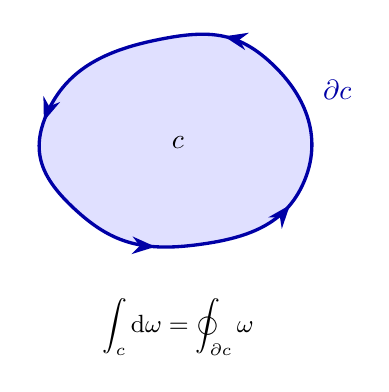
\begin{tikzpicture}[scale=1.0,>=Stealth]
  \fill[blue!12] plot[smooth cycle,tension=0.85]
      coordinates {(0,0) (1.5,-0.45) (2.9,0.35) (2.5,1.85) (1.0,2.15) (-0.35,1.25)};
  \draw[very thick,blue!65!black,
        decoration={markings, mark=at position 0.14 with {\arrow{Stealth}},
                              mark=at position 0.42 with {\arrow{Stealth}},
                              mark=at position 0.70 with {\arrow{Stealth}},
                              mark=at position 0.95 with {\arrow{Stealth}}},
        postaction={decorate}]
      plot[smooth cycle,tension=0.85]
      coordinates {(0,0) (1.5,-0.45) (2.9,0.35) (2.5,1.85) (1.0,2.15) (-0.35,1.25)};
  \node at (1.3,0.85) {$c$};
  \node[blue!65!black,anchor=west] at (3.02,1.52) {$\partial c$};
  \node[font=\small,anchor=north] at (1.3,-1.0) {$\displaystyle\int_c \dd\omega = \oint_{\partial c}\omega$};
\end{tikzpicture}
\hspace{1.1cm}
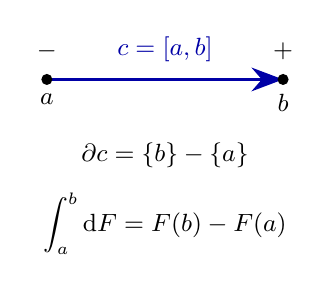
\begin{tikzpicture}[scale=1.0,>=Stealth]
  \draw[very thick,blue!65!black,-{Stealth[length=4mm]}] (0,0.9) -- (3.0,0.9);
  \node[blue!65!black,font=\small,anchor=south] at (1.5,1.0) {$c=[a,b]$};
  \fill (0,0.9) circle (2.0pt);
  \fill (3.0,0.9) circle (2.0pt);
  \node[font=\small,anchor=south] at (0,1.02) {$-$};
  \node[font=\small,anchor=south] at (3.0,1.02) {$+$};
  \node[font=\small,anchor=north,inner sep=4pt] at (0,0.86) {$a$};
  \node[font=\small,anchor=north,inner sep=4pt] at (3.0,0.86) {$b$};
  \node[font=\small,anchor=north,align=center] at (1.5,0.22)
     {$\partial c = \{b\} - \{a\}$};
  \node[font=\small,anchor=north] at (1.5,-0.42)
     {$\displaystyle\int_a^b \dd F = F(b)-F(a)$};
\end{tikzpicture}
\caption{Stokes' theorem. Left: $p=2$, the classical Green/Kelvin picture --- the boundary
of a 2-chain is an oriented loop, with the induced orientation. Right: the degenerate but
most important case $p=1$. A $0$-chain is a finite set of points with signs, and integrating
a $0$-form over it means \emph{evaluating the function and adding with those signs}. Stokes
then reads $F(b)-F(a)$: the fundamental theorem of calculus.}
\label{fig:stokes}
\end{figure}

\subsection{$p=1$: the fundamental theorem of calculus}
\label{sec:ftc}

Take $\M=\R$, $c=[a,b]$, and $\omega=F$ a function. Then $\dd F=F'(x)\dd x$, so
$\int_c\dd F=\int_a^bF'(x)\dd x$; and $\partial c=\{b\}-\{a\}$, with integration of a function
over a point being \emph{evaluation}, $\int_{\{q\}}F:=F(q)$, so $\int_{\partial c}F=F(b)-F(a)$.
Substituting in \eqref{eq:stokes},
\begin{equation}
\boxed{\ \int_a^bF'(x)\,\dd x=F(b)-F(a).\ }
\label{eq:ftc}
\end{equation}

\begin{keybox}
\textbf{Answer to Q8.} $\int\dd x\,f'(x)=F(x)$ is Stokes' theorem in the lowest degree. The
content is not a rule about cancelling $\dd x$; it is that \emph{differentiating the integrand
is dual to taking the boundary of the domain}. A one-dimensional integral of a derivative
collapses to endpoint data because the boundary of an interval \emph{is} its endpoints --- and
Fig.~\ref{fig:riemann}(b) is the picture: the level surfaces crossed in the interior get
crossed back and cancel.
\end{keybox}

\subsection{The other three}

\paragraph{Green's theorem ($p=2$ in $\R^2$).} With $\omega=P\dd x+Q\dd y$, the other terms die
by $\dd x\wedge\dd x=0$ and
\begin{equation}
\dd\omega=\Big(\pd{Q}{x}-\pd{P}{y}\Big)\dd x\wedge\dd y
\quad\Longrightarrow\quad
\iint_S\Big(\pd{Q}{x}-\pd{P}{y}\Big)\dd x\,\dd y=\oint_{\partial S}\big(P\dd x+Q\dd y\big).
\label{eq:green2d}
\end{equation}

\paragraph{Kelvin--Stokes ($p=2$ in $\R^3$).} With $\omega=\A^\flat=A_i\dd x^i$ we have
$\dd\omega=\star(\curl\A)^\flat$, so \eqref{eq:stokes} reads
$\iint_S(\curl\A)\cdot\dd\mathbf S=\oint_{\partial S}\A\cdot\dd\boldsymbol\ell$. The notation
$\dd\mathbf S$ hides the $\flat$ and $\star$; note the ``area vector'' is really a $2$-form,
which is why its direction needs a right-hand rule.

\paragraph{Divergence theorem ($p=3$ in $\R^3$).} With
$\omega=\star\A^\flat=A^1\dd y\wedge\dd z+\text{cyc.}$, $\dd\omega=(\dive\A)\vol$ and
\eqref{eq:stokes} is $\iiint_V(\dive\A)\dd V=\oiint_{\partial V}\A\cdot\dd\mathbf S$.

\begin{keybox}
\textbf{Answer to Q8 (continued).} All four are the single identity
$\int_c\dd\omega=\int_{\partial c}\omega$, differing only in the degree $p$ and in how much
$\flat/\star$ is used to disguise forms as vector fields. The reformulation is not a translation
exercise: it explains why the theorems exist, why they hold in any dimension, and why they need
no metric even though the classical statements are full of dot products and normals.
\end{keybox}

\subsection{Integration by parts, adjoints, and where Green's functions come from}
\label{sec:adjoint}

Apply Stokes to the graded product rule, Definition~\ref{def:extd}(ii), over an $n$-chain:
\begin{equation}
\int_c\dd\alpha\wedge\beta=\int_{\partial c}\alpha\wedge\beta-(-1)^p\int_c\alpha\wedge\dd\beta ,
\label{eq:ibpforms}
\end{equation}
which is \eqref{eq:ibp} in arbitrary degree: \emph{integration by parts is Stokes applied to a
product}. Introduce a metric and an orientation so $\star$ exists, and define the
$L^2$ inner product on $\Om^p(\M)$,
\begin{equation}
(\alpha,\beta):=\int_\M\alpha\wedge\star\beta .
\label{eq:l2}
\end{equation}
Dropping the boundary term in \eqref{eq:ibpforms} gives
$(\dd\alpha,\beta)=(\alpha,\dd^\dagger\beta)$ with $\dd^\dagger=\pm\star\dd\star$: \emph{the
codifferential is not an extra definition, it is the adjoint of $\dd$ forced by Stokes.} So the
subject carries two adjointnesses, worth keeping apart:
\begin{center}\small
\renewcommand{\arraystretch}{1.15}
\begin{tabular}{@{}lll@{}}
\toprule
pairing & adjoint pair & structure needed \\
\midrule
$\pair{c}{\omega}=\int_c\omega$ (domains $\times$ forms) & $\partial$ and $\dd$ & none \\
$(\alpha,\beta)=\int_\M\alpha\wedge\star\beta$ (forms $\times$ forms) & $\dd^\dagger$ and $\dd$
  & metric, orientation \\
\bottomrule
\end{tabular}
\end{center}

\paragraph{And what ``inverse of a differential operator'' means.} To solve $Lu=f$ one wants
$L^{-1}$. But $L$ is local while $L^{-1}$ is not, so $L^{-1}$ cannot be a differential
operator; it is an \emph{integral} operator, and an integral operator is specified by a kernel
$G(x,y)$ \emph{depending on two points}:
\begin{equation}
u(x)=\big(L^{-1}f\big)(x)=\int_{y}G(x,y)\,f(y) .
\label{eq:kernelrep}
\end{equation}
Two consequences. First, \eqref{eq:kernelrep} \emph{is} the statement that $f\mapsto u$ is
linear: for a nonlinear equation there is no kernel, and ``the Green's function'' names nothing.
Superposition and the existence of $G$ are the same fact. Second, the degrees are forced: for
the $y$-integral to make sense, $G$ must carry a top form in $y$, and for the answer to be a
$p$-form in $x$ it must carry that too. The defining equation is
\begin{equation}
L_x\,G(x,y)=\delta(x,y),
\end{equation}
and \S\ref{sec:green} identifies the right-hand side: it is the diagonal $\{x=y\}$ regarded as a
domain, so that ``$\delta$'' is again a chain and $LG=\delta$ says $G$ is the object whose image
under $L$ is the diagonal. \S\ref{sec:green} does the one- and three-dimensional cases
explicitly.


\section{The indefinite integral, and inexact differentials}
\label{sec:exact}

\subsection{Reading $F(x)=\int\dd x\,f(x)$ honestly}

The notation $\int\dd x\,f(x)$ has no domain attached, so by \eqref{eq:pairing} it is not an
integral at all. What is meant is:

\begin{keybox}
\textbf{Answer to Q5.} ``$F=\int\dd x\,f$'' is the request: \emph{given the $1$-form
$\omega=f\,\dd x$, find a function $F$ with $\dd F=\omega$}. It is an equation, not an
operation --- an instance of asking whether $\omega$ is the differential of something. Forms
that are are called \textbf{exact}. So \emph{antidifferentiation is the search for a potential.}
\label{eq:antider}
\end{keybox}

\noindent Two structural facts follow. \emph{Uniqueness}: if $\dd F_1=\dd F_2$ then
$\dd(F_1-F_2)=0$, and a function with vanishing differential is constant on each connected
piece of the domain. The ``$+C$'' of elementary calculus is exactly that freedom --- one
independent constant per connected component, which is the bookkeeping you need when
integrating $1/x$ separately on $x<0$ and $x>0$.

\emph{Existence needs a condition}: since $\dd\dd=0$, a necessary condition is
$\dd\omega=0$, and such forms are called \textbf{closed}. In one variable this is vacuous
(every $2$-form on $\R$ vanishes), which is why every continuous $f$ on an interval has an
antiderivative and the issue is invisible in first-year calculus. In two or more variables it
bites: for $\omega=P\dd x+Q\dd y$,
\begin{equation}
\dd\omega=0\iff\pd{P}{y}=\pd{Q}{x},
\label{eq:integrability}
\end{equation}
which is the classical \emph{integrability condition} --- and \eqref{eq:integrability} is why
your thermodynamics course tested ``exact differentials'' with a cross-derivative check. The
converse holds locally: on a region that can be shrunk to a point, closed forms are exact
(the \emph{Poincar\'e lemma}). Globally it can fail, and that failure is physics.

\subsection{Closed but not exact}
\label{sec:closednotexact}

\begin{ex}[The angle form]\label{ex:dtheta}
On the punctured plane $\M=\R^2\setminus\{0\}$ put
\begin{equation}
\omega=\frac{x\,\dd y-y\,\dd x}{x^2+y^2}.
\end{equation}
A direct computation gives $\dd\omega=0$. On any patch not encircling the origin,
$\omega=\dd\theta$ with $\theta$ a branch of the polar angle --- as the Poincar\'e lemma
promises. But $\omega$ is \emph{not} $\dd$ of any function on all of $\M$: integrating round the
unit circle,
\begin{equation}
\oint_{S^1}\omega=2\pi\ne0 ,
\end{equation}
whereas for an exact form Stokes forces $\oint\dd F=0$ around any closed curve. There is no
global single-valued angle; $\theta$ jumps by $2\pi$.
\end{ex}

\begin{figure}[h]
\centering
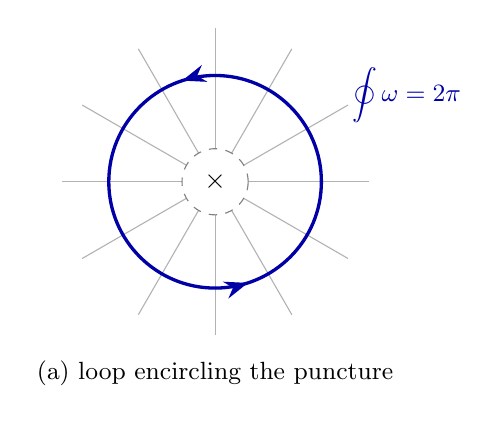
\begin{tikzpicture}[scale=1.0,>=Stealth]
  \foreach \a in {0,30,...,330}{\draw[gray!60] (\a:0.42) -- (\a:1.95);}
  \fill[white] (0,0) circle (0.42);
  \draw[dashed,gray] (0,0) circle (0.42);
  \node at (0,0) {$\times$};
  \draw[very thick,blue!65!black,decoration={markings,
        mark=at position 0.30 with {\arrow{Stealth}},
        mark=at position 0.80 with {\arrow{Stealth}}},postaction={decorate}]
        (0,0) circle (1.35);
  \node[blue!65!black,font=\small,anchor=west] at (1.62,1.10) {$\displaystyle\oint\omega = 2\pi$};
  \node[font=\small,anchor=north] at (0,-2.15) {(a) loop encircling the puncture};
\end{tikzpicture}
\hspace{1.4cm}
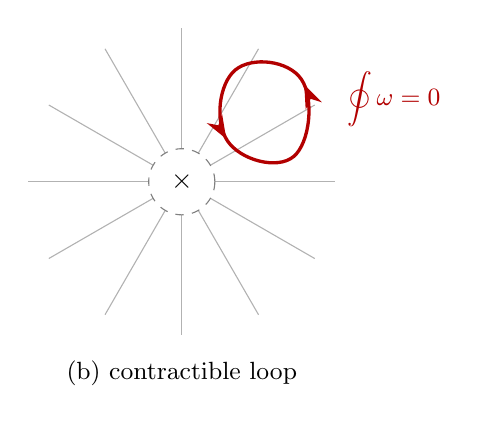
\begin{tikzpicture}[scale=1.0,>=Stealth]
  \foreach \a in {0,30,...,330}{\draw[gray!60] (\a:0.42) -- (\a:1.95);}
  \fill[white] (0,0) circle (0.42);
  \draw[dashed,gray] (0,0) circle (0.42);
  \node at (0,0) {$\times$};
  \draw[very thick,red!70!black,decoration={markings,
        mark=at position 0.25 with {\arrow{Stealth}},
        mark=at position 0.75 with {\arrow{Stealth}}},postaction={decorate}]
        plot[smooth cycle,tension=0.8] coordinates {(0.58,0.52) (1.42,0.32) (1.52,1.30) (0.68,1.42)};
  \node[red!70!black,font=\small,anchor=west] at (1.98,1.05) {$\displaystyle\oint\omega = 0$};
  \node[font=\small,anchor=north] at (0,-2.15) {(b) contractible loop};
\end{tikzpicture}
\caption{The angle form $\omega=\dd\theta$ on the punctured plane
(Ex.~\ref{ex:dtheta}); grey rays are its level surfaces. It is closed, hence locally $\dd$ of
something, so (b) vanishes by Stokes. But (a) cannot be shrunk to a point without crossing the
puncture, the surface count does not cancel, and it returns $2\pi$ --- so no global potential
exists. The same picture, relabelled, is the Aharonov--Bohm phase and the Dirac string.}
\label{fig:dtheta}
\end{figure}

\noindent The number $2\pi$ is the same for \emph{every} loop that encircles the origin once,
and zero for every loop that does not. It is therefore a property of the \emph{hole}, not of the
form or the loop --- a fact about the shape of the region. That is all one needs; there is no
call here for the machinery mathematicians build on top of it.

\begin{keybox}
\textbf{The physics of ``closed but not exact''.}
\begin{itemize}[leftmargin=1.2em,itemsep=2pt]
\item \emph{Conservative forces.} A force $1$-form admits a potential iff it is exact.
      $\dd\omega=0$ is $\curl\mathbf F=0$, and on a region with no holes that is enough. On a
      region with a hole it is not.
\item \emph{Thermodynamics.} $\delta Q$ is not closed: $\oint\delta Q\ne0$ round a cycle,
      which is how an engine does work. The second law supplies an \emph{integrating factor},
      $\delta Q/T=\dd S$ --- see \S\ref{sec:frobenius} for why one can exist.
\item \emph{Electromagnetism.} Outside a solenoid $\B=0$, so $\dd\A^\flat=0$, yet
      $\oint\A\cdot\dd\boldsymbol\ell=\Phi\ne0$: the vector potential is closed and not exact,
      and the Aharonov--Bohm phase $\exp(\tfrac{ie}\hbar\oint\A\cdot\dd\boldsymbol\ell)$ measures
      it. For a magnetic monopole the same happens one degree up, with
      $\int_{S^2}F=4\pi g$, and Dirac's quantisation condition says that number must be an
      integer multiple of a fixed unit.
\end{itemize}
\end{keybox}

\subsection{Inexact differentials: what $\delta Q$ and $\delta W$ are}
\label{sec:inexact}

Thermodynamics writes $\dd U$ for internal energy but $\delta Q$, $\delta W$ for heat and work,
and warns that the latter are ``inexact differentials''. The warning is precise and the notation
is almost right. Let $\Sigma$ be the space of equilibrium states --- a manifold, with $(T,V)$ or
$(U,V)$ or $(S,p)$ as alternative charts on it. Then:

\begin{keybox}
\textbf{$\delta Q$ and $\delta W$ are perfectly ordinary $1$-forms on $\Sigma$. What they are
not is $\dd$ of anything.} The ``$\delta$'' is not an operator; it is a warning label meaning
\emph{there is no function $Q$ on $\Sigma$ whose differential this is}. Writing ``$\dd Q$''
would assert a state function $Q$, which is exactly what is false.
\end{keybox}

\noindent \textbf{So what is $Q$?} Not a function on $\Sigma$, but a number attached to a
\emph{process}, and a quasi-static process is an oriented path --- a domain in the sense of
\S\ref{sec:integration}. By \eqref{eq:pairing},
\begin{equation}
Q[\gamma]:=\int_\gamma\delta Q,\qquad W[\gamma]:=\int_\gamma\delta W .
\label{eq:QW}
\end{equation}
\emph{$U$ is a function on $\Sigma$; $Q$ and $W$ are functions of the path.} That type mismatch
is the whole content of ``heat and work are not state functions''. Asking for the heat of a
state is a category error, like asking for the arclength of a point.

\textbf{Path dependence is the failure of Stokes to collapse.} For the exact form $\dd U$,
Stokes gives $\int_\gamma\dd U=U(\text{final})-U(\text{initial})$: only $\partial\gamma$
matters. For $\delta Q$ there is no such collapse (Fig.~\ref{fig:inexact}a). \emph{Exactness of
the integrand is precisely the condition under which an integral depends only on the boundary of
its domain.}

\textbf{The first law is an equation in $\Om^1(\Sigma)$}: $\delta Q=\dd U+\delta W$, with
$\delta W=p\,\dd V$ for a simple compressible system. Two non-exact $1$-forms differ by an exact
one; nothing is paradoxical, since the exact forms are a linear subspace of $\Om^1$ and the
difference happens to land in it. Note $\dd(p\,\dd V)=\dd p\wedge\dd V\ne0$, so work is
path-dependent too, and becomes computable only once you \emph{specify} the process.

\textbf{Work per cycle is Green's theorem.} For a closed cycle $\gamma=\partial S$ in the
$(V,p)$ plane, $\oint\dd U=0$ always, so $Q=W$ per cycle, and by \eqref{eq:green2d}
\begin{equation}
W_{\text{cycle}}=\oint_{\partial S}p\,\dd V=\int_S\dd p\wedge\dd V=\pm\,\mathrm{Area}(S),
\label{eq:pvarea}
\end{equation}
positive for a clockwise circuit --- which is why engine cycles run clockwise on a $p$--$V$
diagram and the enclosed area is the work output (Fig.~\ref{fig:inexact}b). The ``area under the
curve'' rule of a first thermodynamics course is Green's theorem.

\begin{figure}[h]
\centering
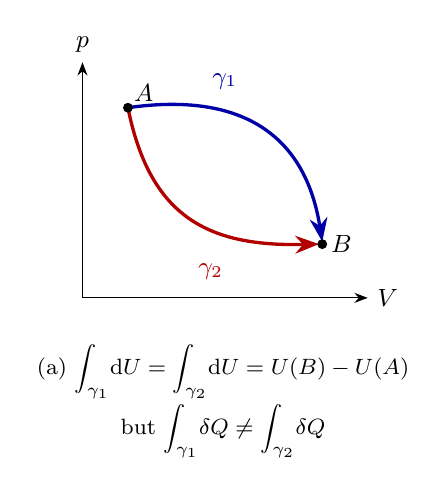
\begin{tikzpicture}[scale=1.05,>=Stealth,font=\small]
  \draw[->] (0,0) -- (3.45,0) node[right]{$V$};
  \draw[->] (0,0) -- (0,2.85) node[above]{$p$};
  \draw[very thick,blue!65!black,-{Stealth[length=3mm]}]
        (0.55,2.30) .. controls (1.95,2.50) and (2.70,1.95) .. (2.90,0.68);
  \draw[very thick,red!70!black,-{Stealth[length=3mm]}]
        (0.55,2.30) .. controls (0.82,0.95) and (1.55,0.62) .. (2.86,0.65);
  \fill (0.55,2.30) circle (1.7pt) node[above right,inner sep=2pt]{$A$};
  \fill (2.90,0.65) circle (1.7pt) node[right,inner sep=3pt]{$B$};
  \node[blue!65!black] at (1.72,2.62) {$\gamma_1$};
  \node[red!70!black]  at (1.55,0.32) {$\gamma_2$};
  \node[anchor=north,align=center,font=\footnotesize] at (1.7,-0.45)
    {(a) $\displaystyle\int_{\gamma_1}\!\dd U=\int_{\gamma_2}\!\dd U = U(B)-U(A)$\\[1pt]
     but $\displaystyle\int_{\gamma_1}\!\delta Q \neq \int_{\gamma_2}\!\delta Q$};
\end{tikzpicture}
\hspace{1.0cm}
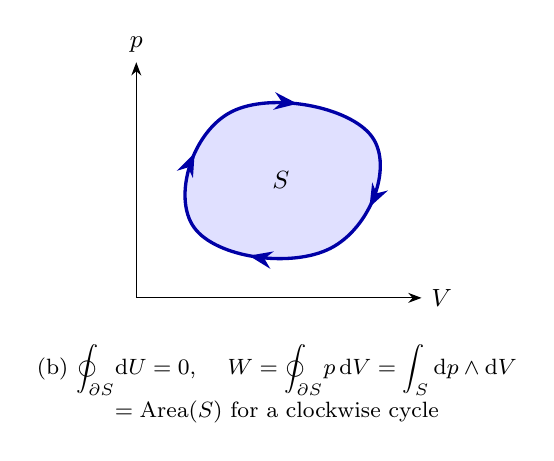
\begin{tikzpicture}[scale=1.05,>=Stealth,font=\small]
  \draw[->] (0,0) -- (3.45,0) node[right]{$V$};
  \draw[->] (0,0) -- (0,2.85) node[above]{$p$};
  \fill[blue!12] plot[smooth cycle,tension=0.8]
     coordinates {(0.70,0.85) (1.15,2.25) (2.85,1.95) (2.35,0.60)};
  \draw[very thick,blue!65!black,decoration={markings,
        mark=at position 0.12 with {\arrow{Stealth}},
        mark=at position 0.40 with {\arrow{Stealth}},
        mark=at position 0.65 with {\arrow{Stealth}},
        mark=at position 0.90 with {\arrow{Stealth}}},postaction={decorate}]
     plot[smooth cycle,tension=0.8]
     coordinates {(0.70,0.85) (1.15,2.25) (2.85,1.95) (2.35,0.60)};
  \node at (1.75,1.42) {$S$};
  \node[anchor=north,align=center,font=\footnotesize] at (1.7,-0.45)
    {(b) $\displaystyle\oint_{\partial S}\!\dd U = 0$, \quad
     $\displaystyle W=\oint_{\partial S}\! p\,\dd V = \int_S \dd p\wedge \dd V$\\[1pt]
     $=\mathrm{Area}(S)$ for a clockwise cycle};
\end{tikzpicture}
\caption{Inexact differentials. (a) $\dd U$ is exact, so its integral collapses onto
$\partial\gamma$ and is the same along both paths; $\delta Q$ is not, so it does not. (b) Around
a closed cycle the exact form integrates to zero, while $\oint p\,\dd V$ equals the enclosed
area by Stokes' theorem in degree $2$ --- the work output of the engine.}
\label{fig:inexact}
\end{figure}

\textbf{Entropy, and the non-uniqueness of $T$.} $\delta Q$ is not exact, but it admits an
integrating factor, traditionally $1/T$, giving $\delta Q/T=\dd S$. The factor is not unique: if
also $\delta Q=\tilde T\dd\tilde S$ then $\dd\tilde S$ is parallel to $\dd S$, so
$\tilde S=g(S)$ and $\tilde T=T/g'(S)$. Geometry gives the \emph{existence} of a temperature and
an entropy; fixing the Kelvin scale picks one representative.

\textbf{All four Maxwell relations are $\dd^2=0$.} Substituting $\delta Q=T\dd S$ and
$\delta W=p\,\dd V$ gives the Gibbs relation $\dd U=T\dd S-p\,\dd V$. Apply $\dd$ and use
$\dd\dd U=0$:
\begin{equation}
\boxed{\ \dd T\wedge\dd S=\dd p\wedge\dd V\ }
\label{eq:maxwellrel}
\end{equation}
a single equation between $2$-forms on the two-dimensional state space. Expand it in the chart
$(T,V)$, writing $\dd S=S_T\dd T+S_V\dd V$ and $\dd p=p_T\dd T+p_V\dd V$ and using
$\dd T\wedge\dd T=\dd V\wedge\dd V=0$:
\begin{equation}
S_V\,\dd T\wedge\dd V=p_T\,\dd T\wedge\dd V
\qquad\Longrightarrow\qquad
\left(\pd{S}{V}\right)_{\!T}=\left(\pd{p}{T}\right)_{\!V},
\end{equation}
and identically in the charts $(T,p)$, $(S,V)$, $(S,p)$:
\begin{equation}
\left(\pd{S}{p}\right)_{\!T}\!=-\left(\pd{V}{T}\right)_{\!p}\!,\qquad
\left(\pd{T}{V}\right)_{\!S}\!=-\left(\pd{p}{S}\right)_{\!V}\!,\qquad
\left(\pd{T}{p}\right)_{\!S}\!=\left(\pd{V}{S}\right)_{\!p}\! .
\end{equation}
The usual derivation invents four potentials ($U,F,H,G$) and cross-differentiates each;
\eqref{eq:maxwellrel} shows the four relations are one statement in four charts, with the minus
signs coming only from the anticommutativity of $\wedge$.

\section{Differential equations in the language of forms}
\label{sec:de}

\subsection{As a geometric condition: when does a potential exist?}
\label{sec:frobenius}

A nowhere-zero $1$-form $\omega$ on $\M^n$ picks out, at each point, the hyperplane
$\Ker\omega_p$ of directions it annihilates --- a field of hyperplanes. The equation
$\omega=0$ asks for surfaces whose tangent planes are those hyperplanes, and that is exactly
what a first-order differential equation asks. On $\R^2$,
\begin{equation}
\frac{\dd y}{\dd x}=f(x,y)\iff\omega:=\dd y-f(x,y)\,\dd x=0 ,
\end{equation}
and a solution is a curve whose tangent $\omega$ sends to zero. Written this way the
equation is manifestly geometric: no choice of independent variable, so vertical tangents cause
no trouble. Whether surfaces of the maximal dimension $n-1$ exist is not automatic.

\begin{thm}[Frobenius]\label{thm:frobenius}
For nowhere-zero $\omega\in\Om^1(\M)$ the following are equivalent: (i) through every point
there is an $(n-1)$-dimensional surface everywhere tangent to $\Ker\omega$; (ii)
$\dd\omega\wedge\omega=0$; (iii) locally $\omega=\mu\,\dd f$ for functions $\mu\ne0$, $f$ ---
i.e.\ $\omega$ admits an \emph{integrating factor}.
\end{thm}

\noindent Condition (iii) says $\omega$ need not be exact, nor even closed, but if
$\dd\omega\wedge\omega=0$ it becomes exact after multiplying by a function, and the solution
surfaces are the level sets of $f$: they \emph{stack} to fill $\M$. If
$\dd\omega\wedge\omega\ne0$ the hyperplanes twist as you move, no surface is everywhere tangent
to them, and the constraint is called \emph{non-holonomic} --- rolling without slipping, or a
skate blade on ice.

\begin{ex}[Entropy exists]\label{ex:entropy}
For a simple system the state space is two-dimensional, say $(U,V)$, and
$\delta Q=\dd U+p\,\dd V$. It is not closed: $\dd\,\delta Q=\partial_Up\;\dd U\wedge\dd V\ne0$.
But $\dd(\delta Q)\wedge\delta Q$ is a $3$-form on a $2$-dimensional space, hence
\emph{identically zero}, so Frobenius guarantees an integrating factor. Calling it $1/T$ gives
$\delta Q/T=\dd S$. For systems with $n\ge3$ independent variables integrability is a genuine
condition, and Carath\'eodory's form of the second law --- ``in every neighbourhood of any state
there are states not reachable adiabatically'' --- is exactly the statement that it holds, whence
$T$ and $S$ exist. \emph{The second law is a Frobenius condition.}
\end{ex}

\subsection{As an operator equation: Maxwell}

The other reading: $\dd$, $\dd^\dagger$, $\star$ and $\wedge$ generate the differential
operators, and a field equation is a statement about forms --- manifestly coordinate-free, with
its integral version following by pairing with a domain and applying Stokes. On spacetime let
$A=A_\mu\dd x^\mu$ be the potential and $F:=\dd A$, so
$F_{\mu\nu}=\partial_\mu A_\nu-\partial_\nu A_\mu$. Then \emph{all four} Maxwell equations are
\begin{equation}
\boxed{\ \dd F=0,\qquad \dd\!\star\!F=J\ }
\qquad J\in\Om^3\ \text{the current $3$-form.}
\label{eq:maxwell}
\end{equation}
Unpacking: $\dd F=0$ (four components) is $\nabla\cdot\B=0$ and
$\partial_t\B+\nabla\times\E=0$; if $F=\dd A$ these hold identically by $\dd^2=0$, and
conversely $\dd F=0$ gives $F=\dd A$ \emph{locally} (Poincar\'e), with global existence
obstructed exactly by a magnetic monopole. Next, $\dd\star F=J$ is Gauss's law and
Amp\`ere--Maxwell; the $\star$ is the only place the metric enters, which is why these two know
about the light cone and the other two do not. Applying $\dd^2=0$ to the second gives
$\dd J=0$: \emph{charge conservation is forced, not assumed}. Gauge invariance
$A\mapsto A+\dd\chi$ leaves $F$ alone, again by $\dd^2=0$ --- the same algebra as the ``$+C$''
of \S\ref{sec:exact}, one degree up. Finally, pairing \eqref{eq:maxwell} with domains recovers
the integral forms: $\int_{\partial V}\star F=\int_VJ$ is Gauss's law with the enclosed charge,
and $\oint_{\partial S}\A\cdot\dd\boldsymbol\ell=\int_SF$ is the flux rule.

\begin{keybox}
\textbf{Answer to Q9a.} A differential equation is either (i) the condition that a surface be
tangent to the kernel of given forms --- solvability is then Frobenius, and geometric; or (ii)
an equation between spaces of forms built from $\dd$, $\dd^\dagger$, $\star$, $\wedge$. Physics
uses both: constraints and thermodynamics are (i), field equations are (ii).
\end{keybox}


\section{Thermodynamics: response functions and transitions}
\label{sec:thermo}

\S\ref{sec:inexact} already put the first law and the Maxwell relations in this language. Three
more payoffs follow, and they need nothing beyond what is above.

\subsection{Sorting the quantities by type}

Most confusions of a first thermodynamics course are type errors. $U,S,V,T,p,F,G,H$ are
\emph{functions} on the state space $\Sigma$: they have values at a state, and differences are
path-independent. $\delta Q$ and $\delta W$ are \emph{$1$-forms}, not exact: no value at a
state, only integrable along a process. $Q[\gamma]$ and $W[\gamma]$ are functions of the
\emph{path}. And $\dd T\wedge\dd S=\dd p\wedge\dd V$ is a $2$-form identity. In particular
\emph{entropy is a function and heat is not}: $S$ exists because Frobenius supplies an
integrating factor (Ex.~\ref{ex:entropy}), and $Q$ does not.

\subsection{Response functions are ratios of covectors in a direction}
\label{sec:response}

Here is the cleanest payoff. Let $\vv$ be the tangent to a process at a state. Using
$\delta Q=T\dd S$,
\begin{equation}
\boxed{\ C(\vv)=\frac{\delta Q(\vv)}{\dd T(\vv)}=T\,\frac{\dd S(\vv)}{\dd T(\vv)}\ }
\label{eq:specheat}
\end{equation}
Both numerator and denominator are \emph{linear} in $\vv$, so $C$ is unchanged by
$\vv\mapsto\lambda\vv$: it depends only on the \emph{direction} of the process. That is exactly
why ``the specific heat'' is not a quantity and $C_V$, $C_p$ are:
\begin{itemize}[leftmargin=1.3em,itemsep=1pt]
\item $C_V$ is $C(\vv)$ in the direction with $\dd V(\vv)=0$; $C_p$ the one with $\dd p(\vv)=0$;
\item on the \emph{adiabatic} direction $\dd S(\vv)=0$, so $C=0$;
\item on the \emph{isothermal} direction $\dd T(\vv)=0$, so $C=\infty$.
\end{itemize}
\emph{The specific heat is a function on the set of process directions, vanishing on the adiabat
and blowing up on the isotherm}; $C_V$ and $C_p$ are two samples of it. The subscript is not
decoration --- it is the missing argument. Every other response function has the same shape,
a response $1$-form over a driving $1$-form along a constrained direction:
\begin{equation}
\kappa_T=-\frac1V\frac{\dd V(\vv)}{\dd p(\vv)}\bigg|_{\dd T(\vv)=0},\quad
\alpha=\frac1V\frac{\dd V(\vv)}{\dd T(\vv)}\bigg|_{\dd p(\vv)=0},\quad
\chi_T=\frac{\dd M(\vv)}{\dd H(\vv)}\bigg|_{\dd T(\vv)=0}.
\end{equation}

\paragraph{Why so many identities.} On a two-dimensional $\Sigma$ the cotangent space is
two-dimensional, so any three of $\dd T,\dd S,\dd p,\dd V$ satisfy a relation
(\S\ref{sec:triple}) and there are two independent relations among the four. Together with
\eqref{eq:maxwellrel} these generate the whole web of thermodynamic identities ---
$C_p-C_V=TV\alpha^2/\kappa_T$ and its relatives. They are not physics; they are linear algebra
in a two-dimensional space.

\paragraph{Response functions are second derivatives.} Substituting
$S=-(\partial G/\partial T)_p$ and $V=(\partial G/\partial p)_T$,
\begin{equation}
C_p=-T\left(\pd{^2G}{T^2}\right)_{\!p},\qquad
\kappa_T=-\frac1V\left(\pd{^2G}{p^2}\right)_{\!T},\qquad
\alpha=\frac1V\pd{^2G}{\partial T\,\partial p},
\end{equation}
so the response functions are the components of the \emph{Hessian} of a potential --- the object
of \S\ref{sec:higher}. Two consequences: thermodynamic stability is definiteness of that Hessian
($C_p>0$, $\kappa_T>0$), and the Hessian defines a metric on $\Sigma$ whose line element
measures the improbability of a fluctuation. \S\ref{sec:phasetrans} is about what happens to it.

\subsection{What quasi-staticness is for}
\label{sec:quasistatic}

$\Sigma$ is the space of \emph{equilibrium} states. A real process passes through
configurations that are not equilibrium states, hence not points of $\Sigma$ at all.

\begin{keybox}
\textbf{Quasi-staticness is the condition that a process be representable as a path in
$\Sigma$.} It is not an idealisation added afterwards; it is what makes the pairing
\eqref{eq:QW} \emph{exist}. If the process is not quasi-static there is no curve to integrate
over, and ``$\int\delta Q$'' has no referent --- not a wrong value, no value.
\end{keybox}

\noindent Three refinements. First, \emph{why ``slowly'' does not mean ``how slowly''}: by
\S\ref{sec:integration}, $\int_\gamma\omega$ is invariant under reparametrisation, so once the
process is a curve in $\Sigma$ the rate drops out of every thermodynamic integral.
Reparametrisation invariance of the integral of a $1$-form is the formal content of
``quasi-static processes do not care how slow you go'' --- and conversely, the reason
thermodynamics has no time variable is that its integrands are $1$-forms rather than functions.
Second, \emph{quasi-static $\ne$ reversible}: the first says $\gamma$ lies in $\Sigma$, the
second additionally that $\delta Q=T\dd S$ along it. A quasi-static process with friction stays
in $\Sigma$ but produces entropy. Third, \emph{the Clausius inequality is about leaving
$\Sigma$}: for a general process $S(\sigma_2)-S(\sigma_1)\ge\int\delta Q/T$, the left side being
well defined because $S$ is a function and only endpoints are needed, the right side needing a
path and therefore fragile. The second law reads: \emph{the exact form always wins}.

\subsection{Why potentials are minimised}
\label{sec:minim}

\begin{keybox}
\textbf{The honest answer first.} The \emph{reason} equilibrium extremises a potential is
statistical, not geometric: $S=k\log\Omega$, and the observed macrostate is the one with
overwhelmingly the most microstates, fluctuations being suppressed as
$P\propto e^{\Delta S/k}$. No amount of geometry produces that. What geometry supplies is the
\emph{structure} of the resulting statement --- and that structure explains the four potentials,
the multipliers and the stability criteria at once.
\end{keybox}

\noindent \textbf{(1) The intensive variables are Lagrange multipliers.} Maximise $S$ subject to
fixed $U$, $V$, $N$. By \S\ref{sec:lagrange} criticality means $\dd S$ is a combination of the
constraint differentials:
\begin{equation}
\dd S=\frac1T\dd U+\frac pT\dd V-\frac\mu T\dd N .
\label{eq:lagmult}
\end{equation}
So $1/T$, $p/T$, $-\mu/T$ are not separately postulated: they are the multipliers, i.e.\ the
components of $\dd S$, and the Gibbs relation \emph{is} the stationarity condition. Two bodies
in thermal contact equilibrate at a common temperature because $\dd(S_1+S_2)$ must vanish on the
constraint direction $\partial_{U_1}-\partial_{U_2}$, which gives $1/T_1=1/T_2$.

\textbf{(2) The four minimum principles are one principle in four charts.} $U$, $F$, $H$, $G$
are different coordinate choices on the same $\Sigma$; which one you extremise is dictated by
what the environment holds fixed, and \eqref{eq:lagmult} is the same equation in each. The
textbook proliferation is a chart artefact, exactly as the four Maxwell relations were.

\textbf{(3) Why the second-derivative test is legitimate.} Criticality is chart-independent,
but ``minimum'' is a statement about the Hessian, and \S\ref{sec:higher} warned that
$\partial_i\partial_j\Phi$ is not a tensor. The escape is the one noted there: the offending
term in \eqref{eq:hesstransf} is proportional to $\partial_k\Phi$, which vanishes at a critical
point. \emph{The Hessian is tensorial exactly where thermodynamics needs it}, which is why
``$C_p>0$ and $\kappa_T>0$'' is a meaningful criterion and not an artefact of using $(T,p)$
rather than $(S,V)$.

\textbf{(4) But convexity is affine, not differential-geometric.} ``Minimum'' needs only
$\dd\Phi=0$ and a positive Hessian. \emph{Convexity} --- which is what licenses the Maxwell
construction and the convex envelope below --- requires being able to average two states,
$\tfrac12(\sigma_1+\sigma_2)$, and a bare manifold has no such operation. Thermodynamics has it
because the extensive variables $(U,V,N,\dots)$ are \emph{additive}: they live in a real vector
space, and combining subsystems adds coordinates. Global stability rests on that linear
structure, not on the differential structure of $\Sigma$ --- which is also why a coexistence tie
line is a straight line.

\subsection{Phase transitions: three ways for the geometry to fail}
\label{sec:phasetrans}

Fix the control parameters as coordinates on a base $B$, say $(T,p)$, and let $g$ be the Gibbs
free energy on it. All of thermodynamics is then in the derivatives of $g$, and the
classification by ``order'' is a classification of \emph{how they degenerate}.

\paragraph{(i) First order: the total differential does not exist.} Across a coexistence curve
$g$ is continuous but $\dd g$ is not --- the two one-sided limits differ --- so by
Definition~\ref{def:diff} \emph{$g$ has no total differential there}: the situation of
Example~\ref{ex:nolinear}, $|x|$ at the origin. Since $S=-(\partial g/\partial T)_p$ and
$V=(\partial g/\partial p)_T$ are components of $\dd g$, both jump, and $L=T_c\Delta S$ is the
latent heat. The graph of $g$ has a crease where two branches cross; equivalently $g$ is
replaced by the \emph{convex envelope} of the two branches, affine along the tie line --- the
Maxwell construction --- and on that segment the Hessian is \emph{zero}, not divergent.

\begin{figure}[h]
\centering
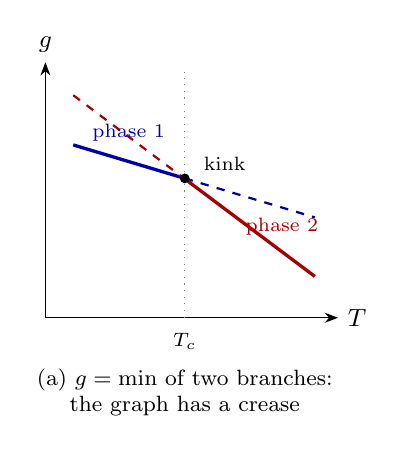
\begin{tikzpicture}[scale=1.18,>=Stealth,font=\small]
  \draw[->] (0,0) -- (3.15,0) node[right]{$T$};
  \draw[->] (0,0) -- (0,2.75) node[above]{$g$};
  \draw[dotted,gray] (1.5,0) -- (1.5,2.65);
  % branch 1: shallower slope, lower for T < Tc
  \draw[thick,blue!60!black,dashed,domain=1.5:2.90,smooth,variable=\x]
       plot ({\x},{1.95-0.30*\x});
  \draw[very thick,blue!65!black,domain=0.30:1.5,smooth,variable=\x]
       plot ({\x},{1.95-0.30*\x});
  % branch 2: steeper slope, lower for T > Tc
  \draw[thick,red!65!black,dashed,domain=0.30:1.5,smooth,variable=\x]
       plot ({\x},{2.62-0.75*\x});
  \draw[very thick,red!65!black,domain=1.5:2.90,smooth,variable=\x]
       plot ({\x},{2.62-0.75*\x});
  \fill (1.5,1.50) circle (1.5pt);
  \node[font=\scriptsize,anchor=west] at (1.60,1.66) {kink};
  \node[blue!65!black,font=\scriptsize,anchor=west] at (0.40,1.99) {phase 1};
  \node[red!65!black,font=\scriptsize,anchor=west]  at (2.05,0.98) {phase 2};
  \node[font=\scriptsize,anchor=north] at (1.5,-0.06) {$T_c$};
  \node[anchor=north,align=center,font=\footnotesize] at (1.5,-0.44)
     {(a) $g=\min$ of two branches:\\ the graph has a crease};
\end{tikzpicture}
\hfill
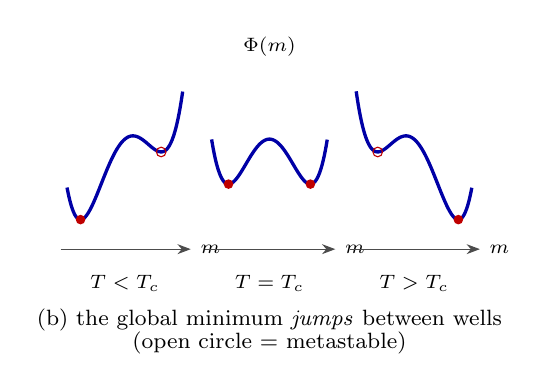
\begin{tikzpicture}[scale=1.02,>=Stealth,font=\small]
  \foreach \lab/\a/\bshift in {{$T<T_c$}/0.26/0, {$T=T_c$}/0.0/1.80, {$T>T_c$}/-0.26/3.60}{
    \begin{scope}[shift={(\bshift,0)}]
      \draw[->,black!70] (-0.80,0) -- (0.82,0) node[right,font=\scriptsize,black]{$m$};
      \draw[very thick,blue!65!black,domain=-0.72:0.72,smooth,samples=90,variable=\x]
        plot ({\x},{1.37+8.32*\x*\x*\x*\x-4.32*\x*\x+3.2*\a*\x});
      \node[font=\scriptsize,anchor=north] at (0,-0.20) {\lab};
    \end{scope}
  }
  % filled = global minimum, open = metastable
  \fill[red!75!black] (-0.552,0.368) circle (1.7pt);
  \draw[red!75!black] (0.452,1.210) circle (1.7pt);
  \fill[red!75!black] (1.80-0.510,0.810) circle (1.7pt);
  \fill[red!75!black] (1.80+0.510,0.810) circle (1.7pt);
  \fill[red!75!black] (3.60+0.552,0.368) circle (1.7pt);
  \draw[red!75!black] (3.60-0.452,1.210) circle (1.7pt);
  \node[anchor=north,align=center,font=\footnotesize] at (1.80,-0.62)
     {(b) the global minimum \emph{jumps} between wells\\[-1pt]
      (open circle $=$ metastable)};
  \node[font=\scriptsize,anchor=south] at (1.80,2.28) {$\Phi(m)$};
\end{tikzpicture}
\caption{Mechanism of a \textbf{first-order} transition. (a) Two branches
cross, so the physical $g$ (solid, the lower one) has a crease at $T_c$: the slopes differ, so
$S=-(\partial g/\partial T)_p$ jumps and $\dd g$ has no limit --- Example~\ref{ex:nolinear} in
disguise. Dashed continuations are the metastable branches (superheating, supercooling). (b) The
same in the Landau potential: two minima exchange depth and the order parameter \emph{jumps}
across a finite gap.}
\label{fig:firstorder}
\end{figure}

\paragraph{(ii) Continuous: the Hessian degenerates.} If $\dd g$ is continuous but the
second-order data is not, the transition is continuous. (Ehrenfest called this ``second
order''; real critical points usually have \emph{divergent} rather than merely discontinuous
second derivatives, which is why the higher Ehrenfest labels are no longer used.) By
\S\ref{sec:response} the second-order data \emph{is} the response functions, so at a critical
point $C_p$, $\kappa_T$, $\chi_T$ diverge. Equivalently: $\Hess g$ acquires a zero eigenvalue,
whose eigenvector is the direction of the \emph{soft mode}\footnote{A \emph{soft mode} is a
fluctuation direction whose restoring force vanishes: an eigenvalue of the Hessian of the free
energy goes to zero, so the corresponding susceptibility and mean-square fluctuation diverge
while the mode's characteristic frequency, or inverse relaxation time, goes to zero. At a
continuous transition it is the order-parameter direction that softens, which is why $C_p$,
$\kappa_T$, $\chi_T$ and $\xi$ all diverge together.}; the map from $\Sigma$ to the control plane
$B$ stops being invertible, by \eqref{eq:invfn}, and the generic failures are the \emph{fold}
and the \emph{cusp}. A van der Waals isotherm is exactly a fold --- the $S$-shape, whose two
turning points are the spinodal, where $\kappa_T$ diverges --- and as $T\to T_c$ the two folds
merge into a cusp, the fold interval shrinks to zero, the latent heat vanishes, and the
transition becomes continuous.

\begin{figure}[h]
\centering
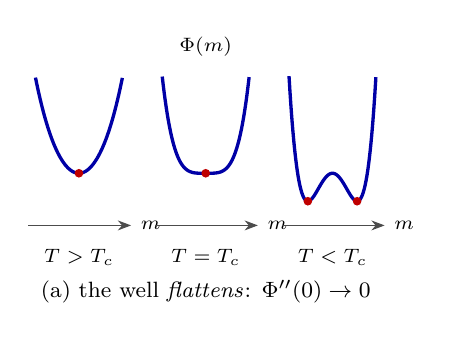
\begin{tikzpicture}[scale=0.92,>=Stealth,font=\small]
  \foreach \lab/\qq/\pp/\bshift in
      {{$T>T_c$}/{3.20}/{1.30}/0, {$T=T_c$}/{0.0}/{10.3}/1.75, {$T<T_c$}/{-6.68}/{28.9}/3.50}{
    \begin{scope}[shift={(\bshift,0)}]
      \draw[->,black!70] (-0.70,0) -- (0.72,0) node[right,font=\scriptsize,black]{$m$};
      \draw[very thick,blue!65!black,domain=-0.60:0.60,smooth,samples=90,variable=\x]
        plot ({\x},{0.72+\pp*\x*\x*\x*\x+\qq*\x*\x});
      \node[font=\scriptsize,anchor=north] at (0,-0.20) {\lab};
    \end{scope}
  }
  \fill[red!75!black] (0,0.72) circle (1.7pt);
  \fill[red!75!black] (1.75,0.72) circle (1.7pt);
  \fill[red!75!black] (3.50-0.34,0.334) circle (1.7pt);
  \fill[red!75!black] (3.50+0.34,0.334) circle (1.7pt);
  \node[font=\scriptsize,anchor=south] at (1.75,2.20) {$\Phi(m)$};
  \node[anchor=north,align=center,font=\footnotesize] at (1.75,-0.62)
     {(a) the well \emph{flattens}: $\Phi''(0)\to0$};
\end{tikzpicture}
\hfill
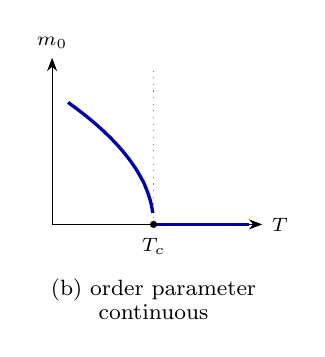
\begin{tikzpicture}[scale=0.92,>=Stealth,font=\small]
  \draw[->] (0,0) -- (2.90,0) node[right,font=\scriptsize]{$T$};
  \draw[->] (0,0) -- (0,2.30) node[above,font=\scriptsize]{$m_0$};
  \draw[dotted,gray] (1.40,0) -- (1.40,2.20);
  \draw[very thick,blue!65!black,domain=0.22:1.39,smooth,samples=70,variable=\x]
       plot ({\x},{1.55*pow(1.40-\x,0.5)});
  \draw[very thick,blue!65!black] (1.40,0) -- (2.72,0);
  \fill (1.40,0) circle (1.4pt);
  \node[font=\scriptsize,anchor=north] at (1.40,-0.06) {$T_c$};
  \node[anchor=north,align=center,font=\footnotesize] at (1.40,-0.62)
     {(b) order parameter\\[-1pt] continuous};
\end{tikzpicture}
\hfill
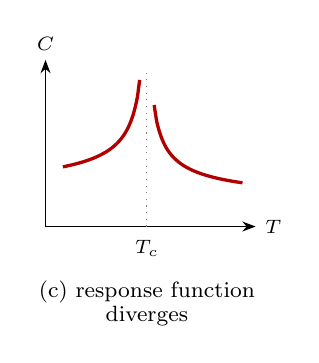
\begin{tikzpicture}[scale=0.92,>=Stealth,font=\small]
  \draw[->] (0,0) -- (2.90,0) node[right,font=\scriptsize]{$T$};
  \draw[->] (0,0) -- (0,2.30) node[above,font=\scriptsize]{$C$};
  \draw[dotted,gray] (1.40,0) -- (1.40,2.20);
  \draw[very thick,red!70!black,domain=0.24:1.30,smooth,samples=70,variable=\x]
       plot ({\x},{0.40+0.46/pow(1.40-\x,0.55)});
  \draw[very thick,red!70!black,domain=1.50:2.72,smooth,samples=70,variable=\x]
       plot ({\x},{0.26+0.40/pow(\x-1.40,0.55)});
  \node[font=\scriptsize,anchor=north] at (1.40,-0.06) {$T_c$};
  \node[anchor=north,align=center,font=\footnotesize] at (1.40,-0.62)
     {(c) response function\\[-1pt] diverges};
\end{tikzpicture}
\caption{Mechanism of a \textbf{continuous} transition. (a) The Landau
potential keeps one minimum until $T_c$, where the quadratic term vanishes and the well becomes
quartic: the Hessian acquires a zero eigenvalue --- a soft mode --- and below $T_c$ the minimum
splits and moves away continuously. (b) So the order parameter is continuous, with infinite
slope: no jump, hence no latent heat. (c) But the response functions \emph{are} the second
derivatives (\S\ref{sec:response}), so a vanishing eigenvalue shows up as a divergence.}
\label{fig:continuous}
\end{figure}

\paragraph{(iii) Infinite order: nothing fails locally.} At a Kosterlitz--Thouless transition
the correlation length diverges as $\xi\sim\exp\big(b/\sqrt{T-T_c}\big)$, so \emph{every}
derivative of $g$ is continuous at $T_c$ and no order of differentiation detects the transition.
The differential geometry of $g$ is blind to it --- because the transition is not in $g$.

What changes is which \emph{shapes} of configuration are available. The order parameter is a
phase, i.e.\ locally a function $\vartheta$, and the physical object is the $1$-form
$\dd\vartheta$ on the plane \emph{with the vortex cores removed}: precisely the angle form of
Example~\ref{ex:dtheta}, closed but not exact, with
\begin{equation}
\frac1{2\pi}\oint_\gamma\dd\vartheta\;\in\;\Z
\end{equation}
the vortex charge enclosed by $\gamma$. Below $T_c$ vortices are bound in neutral pairs and
every large loop returns zero; above $T_c$ they unbind and isolated vortices become
thermodynamically available. \emph{An infinite-order transition is a change in which winding
numbers occur}, invisible to any derivative --- and it is why the closed-but-not-exact material
of \S\ref{sec:closednotexact} is physics and not decoration.

\begin{figure}[h]
\centering
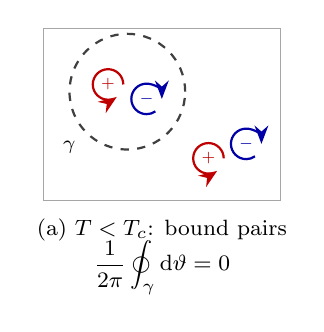
\begin{tikzpicture}[scale=1.02,>=Stealth,font=\small]
  \draw[black!35] (0.10,0.15) rectangle (3.05,2.30);
  % bound pair 1
  \draw[->,red!75!black,thick]  (0.90,1.60) ++(0:0.19) arc (0:305:0.19);
  \node[red!75!black,font=\tiny] at (0.90,1.60) {$+$};
  \draw[<-,blue!65!black,thick] (1.38,1.42) ++(0:0.19) arc (0:305:0.19);
  \node[blue!65!black,font=\tiny] at (1.38,1.42) {$-$};
  % bound pair 2
  \draw[->,red!75!black,thick]  (2.15,0.68) ++(0:0.19) arc (0:305:0.19);
  \node[red!75!black,font=\tiny] at (2.15,0.68) {$+$};
  \draw[<-,blue!65!black,thick] (2.62,0.86) ++(0:0.19) arc (0:305:0.19);
  \node[blue!65!black,font=\tiny] at (2.62,0.86) {$-$};
  % loop
  \draw[dashed,thick,black!75] (1.14,1.51) circle (0.72);
  \node[font=\scriptsize,anchor=north east,fill=white,inner sep=1pt] at (0.54,0.94) {$\gamma$};
  \node[anchor=north,align=center,font=\footnotesize] at (1.57,0.05)
     {(a) $T<T_c$: bound pairs\\[-1pt]
      $\displaystyle\frac{1}{2\pi}\oint_\gamma \dd\vartheta = 0$};
\end{tikzpicture}
\hspace{0.9cm}
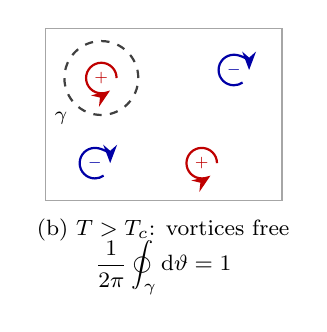
\begin{tikzpicture}[scale=1.02,>=Stealth,font=\small]
  \draw[black!35] (0.10,0.15) rectangle (3.05,2.30);
  \draw[->,red!75!black,thick]  (0.80,1.68) ++(0:0.19) arc (0:305:0.19);
  \node[red!75!black,font=\tiny] at (0.80,1.68) {$+$};
  \draw[<-,blue!65!black,thick] (2.45,1.78) ++(0:0.19) arc (0:305:0.19);
  \node[blue!65!black,font=\tiny] at (2.45,1.78) {$-$};
  \draw[->,red!75!black,thick]  (2.05,0.62) ++(0:0.19) arc (0:305:0.19);
  \node[red!75!black,font=\tiny] at (2.05,0.62) {$+$};
  \draw[<-,blue!65!black,thick] (0.72,0.62) ++(0:0.19) arc (0:305:0.19);
  \node[blue!65!black,font=\tiny] at (0.72,0.62) {$-$};
  \draw[dashed,thick,black!75] (0.80,1.68) circle (0.46);
  \node[font=\scriptsize,anchor=north east,fill=white,inner sep=1pt] at (0.42,1.30) {$\gamma$};
  \node[anchor=north,align=center,font=\footnotesize] at (1.57,0.05)
     {(b) $T>T_c$: vortices free\\[-1pt]
      $\displaystyle\frac{1}{2\pi}\oint_\gamma \dd\vartheta = 1$};
\end{tikzpicture}
\caption{Mechanism of an \textbf{infinite-order} (Kosterlitz--Thouless) transition,
which no derivative of $g$ can see. The order parameter is a phase, so the object of interest is
the closed-but-not-exact $1$-form $\dd\vartheta$ on the plane punctured at the vortex cores ---
the angle form of Example~\ref{ex:dtheta} --- and $\frac1{2\pi}\oint_\gamma\dd\vartheta$ is the
enclosed winding number. (a) Below $T_c$ vortices are bound in neutral pairs, so every large
loop returns zero. (b) Above $T_c$ they unbind and loops return nonzero winding.}
\label{fig:kt}
\end{figure}

\begin{keybox}
\textbf{Summary.} \emph{First order}: $\dd g$ fails to exist --- order-parameter jump, latent
heat, two branches, convex envelope. \emph{Continuous}: $\dd g$ exists, $\Hess g$ degenerates
or diverges --- response functions blow up, the projection to the control plane has a cusp.
\emph{Infinite order}: all derivatives of $g$ are fine; the transition is a change of winding
sector, and only the shape of the configuration space sees it. The three cases are failures of
the first derivative, of the second, and of none --- which is also the order in which
\S\ref{sec:diffable}, \S\ref{sec:higher} and \S\ref{sec:closednotexact} introduced the
machinery.
\end{keybox}


\section{Mean field, Landau--Ginzburg, and where both break}
\label{sec:meanfield}

\S\ref{sec:thermo} treated the state space as given; statistical mechanics has to produce it,
and the standard route has a clean skeleton worth having, because it says precisely what each
approximation discards.

\subsection{Mean field is a restriction to a small family of trial states}
\label{sec:mfrestrict}

Let $\mathcal P$ be the space of probability distributions over configurations. On it the free
energy is an honest \emph{function},
$F[\rho]=\langle H\rangle_\rho-TS[\rho]$, and the Gibbs variational principle says the true
equilibrium state is its minimum, with $\dd F=0$ there. That is \S\ref{sec:minim}, and finding
it exactly is the original many-body problem.

\begin{keybox}
\textbf{Mean field: pick a small family of trial states and minimise inside it.} Take the
product (factorised) distributions $\rho=\bigotimes_i\rho_i(m_i)$, a finite-dimensional surface
$\mathcal N\subset\mathcal P$ whose \emph{coordinates} are the local magnetisations $m_i$. Mean
field replaces $\dd F=0$ by
\begin{equation}
\dd F(\vv)=0\quad\text{for every }\vv\text{ tangent to }\mathcal N,
\qquad\text{but}\qquad \dd F\ne0 .
\label{eq:mfcrit}
\end{equation}
\emph{The self-consistency equations of mean-field theory are the Lagrange condition
\eqref{eq:lagrangian} for a constrained critical point}, with $\mathcal N$ as the constraint.
\end{keybox}

\noindent Three consequences, and they are the whole content of the method.

\emph{(1) What is discarded is named.} At the mean-field solution $\dd F$ still fails to
vanish --- but only in directions that lead off $\mathcal N$. No metric is needed to say that;
what needs a metric is asking how \emph{big} the leftover is, which is \S\ref{sec:mfbreak}.

\emph{(2) The Bogoliubov inequality is trivial.} A minimum over a subset cannot be lower than
the minimum over everything, so $F_{\mathrm{MF}}\ge F_{\mathrm{exact}}$: mean field is a
variational \emph{upper} bound for any choice of $\mathcal N$, and improving it means enlarging
$\mathcal N$.

\emph{(3) When it is exact.} \emph{Precisely when the true minimiser lies on $\mathcal N$}, and
asymptotically when it approaches it: infinite coordination number $z\to\infty$, infinite-range
interactions, large $N$, or high dimension. These are not separate miracles; each says the exact
state becomes a product state.

\begin{figure}[h]
\centering
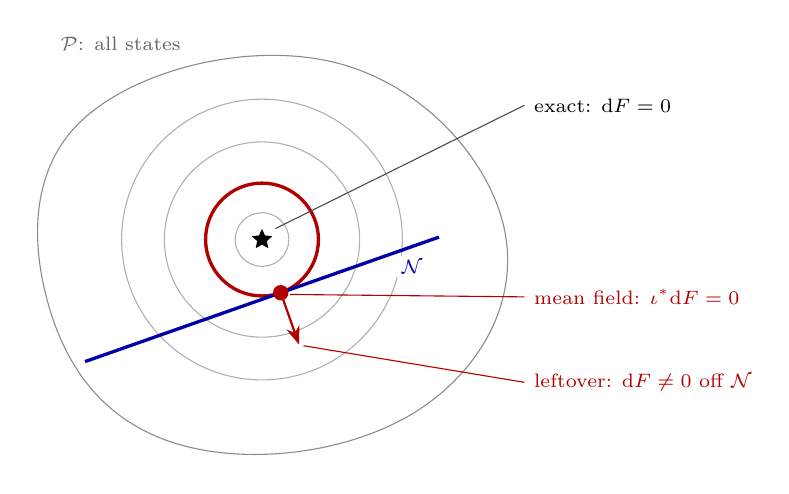
\begin{tikzpicture}[scale=1.55,>=Stealth,font=\small]
  % ambient space of states
  \draw[black!45] plot[smooth cycle,tension=0.72]
     coordinates {(0.02,0.85) (1.15,-0.25) (3.10,0.10) (3.72,1.60) (2.35,2.90) (0.30,2.45)};
  \node[black!60,font=\scriptsize,anchor=south west] at (0.02,2.92)
       {$\mathcal{P}$: all states};
  % level sets of F, the tangent one highlighted
  \foreach \r in {0.22,0.80,1.15}{ \draw[gray!62] (1.75,1.45) circle (\r); }
  \draw[very thick,red!70!black] (1.75,1.45) circle (0.4623);
  % trial submanifold
  \draw[very thick,blue!65!black] (0.30,0.45) -- (3.20,1.47);
  \node[blue!65!black,font=\scriptsize,anchor=north,fill=white,inner sep=1.5pt]
       at (2.98,1.32) {$\mathcal{N}$};
  % exact minimum
  \node[star,star points=5,star point ratio=2.1,fill=black,inner sep=1.3pt] at (1.75,1.45) {};
  % mean-field point and the leftover covector
  \fill[red!70!black] (1.9036,1.0140) circle (1.8pt);
  \draw[->,thick,red!70!black] (1.9036,1.0140) -- (2.053,0.590);
  % annotations, all outside the blob
  \node[font=\scriptsize,anchor=west] (Le) at (3.90,2.55) {exact: $\dd F=0$};
  \draw[thin,black!70] (Le.west) -- (1.86,1.54);
  \node[red!70!black,font=\scriptsize,anchor=west] (Lm) at (3.90,0.98)
       {mean field: $\iota^*\dd F=0$};
  \draw[thin,red!70!black] (Lm.west) -- (1.98,1.00);
  \node[red!70!black,font=\scriptsize,anchor=west] (Ll) at (3.90,0.28)
       {leftover: $\dd F\ne0$ off $\mathcal{N}$};
  \draw[thin,red!70!black] (Ll.west) -- (2.09,0.58);
\end{tikzpicture}
\caption{Mean field as constrained minimisation. Grey circles are level sets
of the free energy $F$ on the space $\mathcal P$ of all states; the star is the exact
equilibrium state, where $\dd F=0$. The blue line is the trial family $\mathcal N$ of product
states, coordinatised by the magnetisations. Mean field finds the point of $\mathcal N$ where a
level set is \emph{tangent} to it --- the same condition as Fig.~\ref{fig:lagrange}. There
$\dd F$ vanishes along $\mathcal N$ but not off it, and the residual is the correlation physics
that is being discarded.}
\label{fig:meanfield}
\end{figure}

\subsection{Landau: the potential is what symmetry allows}
\label{sec:landau}

Mean field delivers a function of the order parameter; Landau stops asking where it came from
and writes the most general one allowed by symmetry. If $G$ is the symmetry group of the
disordered phase and $H$ the subgroup surviving in the ordered phase, the possible values of the
order parameter form the space
\begin{equation}
N=G/H ,
\label{eq:opspace}
\end{equation}
since two states related by an element of $H$ are the same state. The Landau potential $V$ is a
$G$-invariant function on $N$, expanded about the symmetric point --- and by
\S\ref{sec:higher} that expansion is Taylor data, meaningful because we expand about a critical
point.

\begin{keybox}
\textbf{The Landau expansion is the $G$-invariant part of the Taylor expansion of $V$.} For
$G=\Z_2$ acting as $m\mapsto-m$, invariance kills every odd coefficient and leaves
$V(m)=\tfrac12rm^2+\tfrac14um^4+\cdots$ with $r\propto(T-T_c)$; truncating at fourth order
means keeping Taylor data to fourth order. \emph{Which} terms are allowed is a symmetry
question. Nothing is derived --- Landau theory classifies possible shapes, which is why it is
phenomenological and why it is universal.
\end{keybox}

\noindent The Landau function $\Phi(m)$ (free energy at fixed order parameter) and the
measurable $g(h)$ (free energy at fixed conjugate field) are Legendre transforms of each other,
with the equation of state $h=\partial\Phi/\partial m$. Because a Legendre transform is
automatically convex, Landau's non-convex double well is not a defect: the transform
\emph{convexifies}, the flat piece of the envelope is the coexistence tie line, and the Maxwell
construction is built in.

\subsection{Ginzburg: the order parameter is a map, and the gradient term is its length}
\label{sec:ginzburg}

Landau's $m$ is a number. Ginzburg lets it vary in space, and the geometry becomes unavoidable:
with $M$ the sample and $N=G/H$ the order-parameter space, a configuration is a \emph{map}
$\varphi:M\to N$, and its derivative is the tangent map of \S\ref{sec:tangentmap} --- a
$1$-form on $M$ with values in the tangent spaces of the target. The functional is
\begin{equation}
F[\varphi]=\tfrac12\|\dd\varphi\|^2+\int_MV(\varphi)\,\vol_g,
\qquad
\|\dd\varphi\|^2=\int_Mh_{ab}\,\dd\varphi^a\wedge\star\,\dd\varphi^b ,
\label{eq:lgfunctional}
\end{equation}
where $\|\cdot\|$ is the $L^2$ norm \eqref{eq:l2}.

\begin{keybox}
\textbf{The Ginzburg gradient term is the length-squared of the derivative of the order
parameter} --- the only natural quadratic in $\dd\varphi$. Note what it costs: a metric on $M$
(inside $\star$) \emph{and} one on the target $N$. The Landau potential needs neither. So the
split of \eqref{eq:lgfunctional} into ``gradient'' and ``potential'' is the split into the
metric-dependent and metric-free parts, and the stiffness is just the scale of the target
metric.
\end{keybox}

\noindent Varying \eqref{eq:lgfunctional} gives $\Delta\varphi=V'(\varphi)$ for a flat target
with one component. If $G$ is a \emph{local} symmetry, $\dd\varphi$ must be replaced by a
covariant derivative $D\varphi=\dd\varphi-\mathrm{i}qA\varphi$ built from a connection $A$, with
$F=\dd A$; that is the Ginzburg--Landau functional of superconductivity. Deep inside the
superconductor $D\varphi=0$ forces $A=q^{-1}\dd\chi$ with $\varphi=|\varphi|e^{\mathrm i\chi}$,
and single-valuedness gives $\oint\dd\chi=2\pi n$, hence by Stokes
\begin{equation}
\int_SF=\oint_{\partial S}A=\frac{2\pi n}{q},\qquad n\in\Z:
\label{eq:fluxquant}
\end{equation}
\emph{flux quantisation is the same closed-but-not-exact statement as the Dirac condition of
\S\ref{sec:closednotexact}}.

\paragraph{Which defects exist is decided by the shape of $N$.} A defect is a place where
$\varphi$ cannot be extended continuously, so its classification is a question about $N$ alone:
encircle the defect by a small sphere and ask how the map $\varphi$ restricted to it can wrap
around $N$.
\begin{center}\small
\renewcommand{\arraystretch}{1.18}
\begin{tabular}{@{}L{0.235\textwidth}L{0.165\textwidth}L{0.10\textwidth}L{0.39\textwidth}@{}}
\toprule
\textbf{system} & $G\to H$ & $N=G/H$ & \textbf{defects} \\
\midrule
Ising magnet         & $\Z_2\to1$              & two points & domain walls \\
XY model, superfluid & $U(1)\to1$              & circle     & quantised vortices, winding $\in\Z$ \\
Heisenberg magnet    & $SO(3)\to SO(2)$        & sphere     & no stable lines; point defects (hedgehogs) \\
uniaxial nematic     & $SO(3)\to D_{\infty h}$ & sphere with antipodes identified & half-integer disclinations \\
superconductor       & $U(1)$ gauged           & circle     & flux tubes, \eqref{eq:fluxquant} \\
\bottomrule
\end{tabular}
\end{center}
\noindent The circle row is Example~\ref{ex:dtheta} and Fig.~\ref{fig:kt}: the winding
$\frac1{2\pi}\oint\dd\vartheta\in\Z$ \emph{is} the classification, and the closed-but-not-exact
angle form is the whole mechanism. That the nematic's target has antipodes identified is why its
disclinations carry \emph{half}-integer strength --- a prediction made with no dynamics at all.

\subsection{Correlations: $\xi$ comes from a Green's function}

Expand \eqref{eq:lgfunctional} about a uniform solution to second order in the fluctuation. The
two-point correlation function is then the \emph{Green's function} of the resulting operator,
i.e.\ by \S\ref{sec:adjoint} the inverse of $-c\Delta+r$ with $r=V''(\bar\varphi)$:
\begin{equation}
\big(-c\Delta+r\big)G=\delta ,
\qquad
G(x)=\frac{e^{-|x|/\xi}}{4\pi c|x|}\ \ (d=3),
\qquad \xi=\sqrt{c/r} .
\label{eq:yukawa}
\end{equation}
\begin{keybox}
\textbf{Criticality is where that inverse stops existing.} The operator $-c\Delta+r$ has
smallest eigenvalue $r$, so $G$ exists while $r>0$ and its kernel decays with
$\xi=\sqrt{c/r}$. As $T\to T_c$, $r\to0$: the gap closes, $G$ loses its exponential and becomes
a power law with \emph{no length scale}, which is scale invariance. This is
\S\ref{sec:adjoint} again --- an operator ceases to be invertible exactly when it acquires a
zero mode --- and \eqref{eq:yukawa} degenerating to the Coulomb kernel of
\S\ref{sec:laplacegreen} is that limit.
\end{keybox}

\subsection{Breakdown: the mode you kept goes soft}
\label{sec:mfbreak}

\begin{keybox}
\textbf{Mean field assumes the neglected fluctuations are small, and the critical point is
exactly where the mode it \emph{did} keep goes soft.} At $T_c$ the Hessian degenerates
($r\to0$), so by \eqref{eq:yukawa} the fluctuation propagator diverges --- and corrections to
mean field are organised \emph{by} that propagator. The expansion parameter blows up precisely
where the approximation is being used. Mean field fails not because the discarded directions
grow, but because the retained one becomes soft, and softness is what makes the discarded
directions matter.
\end{keybox}

\noindent Quantitatively, with $V=\tfrac12rm^2+\tfrac14um^4$ the ordered value is
$\bar\varphi^2=|r|/u\sim\xi^{-2}$, while the soft modes in the shell $k\lesssim\xi^{-1}$
contribute
\begin{equation}
\big\langle\delta\varphi^2\big\rangle=\int\!\frac{\dd^dk}{(2\pi)^d}\frac{1}{ck^2+|r|}\sim\xi^{\,2-d}
\qquad\Longrightarrow\qquad
\frac{\langle\delta\varphi^2\rangle}{\bar\varphi^{\,2}}\sim\xi^{\,4-d} ,
\label{eq:ginzburgcrit}
\end{equation}
which vanishes as $\xi\to\infty$ iff $d>4$. Hence $d_c=4$: \emph{mean field is
self-consistent above four dimensions and fails below}. Read \eqref{eq:ginzburgcrit}
geometrically --- the \emph{number} of soft modes grows like the volume $\xi^{-d}$ of the soft
shell, each contributing amplitude $\sim\xi^2$, and that must be weighed against the stiffness
$\bar\varphi^2\sim\xi^{-2}$. The critical dimension is where the two counts balance. Nothing
about the failure is mysterious: it is $4-d$.

Below $d_c$ no finite-dimensional trial family will do, and the object of study becomes a
\emph{flow} on the space of couplings --- the renormalisation group. A scale-invariant theory is
a zero of that flow, and the critical exponents are the eigenvalues of its linearisation there.
Those eigenvalues are honest, coordinate-independent numbers for the same reason the Hessian was
tensorial at a critical point (\S\ref{sec:higher}): the inhomogeneous term in the transformation
law is proportional to the flow itself, which vanishes at a zero. Above $d_c$ the mean-field
exponents $\beta=\tfrac12$, $\gamma=1$, $\nu=\tfrac12$ are exact --- so mean field is not a
crude approximation that sometimes works, it is the \emph{exact} answer at one fixed point, and
the question is only whether your system flows there.

\subsection{Mean field in the space of Green's functions}
\label{sec:mfgreen}

Field theory phrases all of this through Green's functions, and doing so sorts out four things
that all get called ``approximations'' but are not the same kind of object.

\paragraph{First, what space.} All the content of an equilibrium propagator sits in its spectral
function: every admissible $G$ has the form
$G(z)=\int\dd\omega\,A(\omega)/(z-\omega)$ with $A\ge0$ and $\int A=1$ (positivity because $A$
is a sum of squared matrix elements, normalisation from the anticommutator sum rule). So the
space $\mathcal G$ of Green's functions is the set of normalised, non-negative spectral
functions: \emph{convex} but not a vector space, with the sharp ones
$A=\delta(\omega-\varepsilon)$ --- the free propagators --- as its extreme points, and
interactions broadening $A$ and moving $G$ inside. A displacement in $\mathcal G$ is a
reshuffling of spectral weight with $\int\delta A=0$.

\begin{keybox}
\textbf{Is a Green's function like $\dd x^i$, i.e.\ a covector?} It has two roles and only one
is. \emph{As a derivative of $W[J]=\ln Z[J]$}: yes --- the one-point function $\delta W/\delta J$
is literally a covector on the space of sources, and the two-point function is a symmetric
bilinear form on it, the analogues of $\dd f$ and the Hessian. \emph{In the variational calculus
below}: no --- there the full $G$ is a \emph{point} of $\mathcal G$, and the covector paired with
it is the \textbf{self-energy} $\Sigma$. The analogue of $\dd x^i$ is $\Sigma$, not $G$, which
is why $(G,\Sigma)$ is the conjugate pair just as $(m,h)$ and $(S,T)$ were.
\end{keybox}

\paragraph{Second, $W[J]$ and its Taylor coefficients.} Expanding $W[J]=\ln Z[J]$ in powers of
the \emph{source} produces the $n$-point functions as coefficients \cite{Greiner}:
\begin{equation}
W[J]=\sum_n\frac1{n!}\int\!\dd^4x_1\cdots\dd^4x_n\;G^{(n)}(x_1,\dots,x_n)J(x_1)\cdots J(x_n).
\label{eq:volterra}
\end{equation}
\emph{This is a definition, not an approximation}: it is the same bookkeeping as writing a
function of several variables as a Taylor series. Expanding in the source is not perturbation
theory. Legendre transforming, with $\bar\varphi:=\delta W/\delta J$ and
$\Gamma[\bar\varphi]:=\int J\bar\varphi-W[J]$, gives $\delta\Gamma/\delta\bar\varphi=J$ --- two
terms cancel in the differentiation precisely because $\bar\varphi$ \emph{is} $\delta W/\delta
J$, the same cancellation as the shadow-price relation \eqref{eq:envelope} --- and at $J=0$ this
is the quantum equation of motion. Two convexity facts follow, worth separating because they are
proved differently: $W$ is convex because $\delta^2W/\delta J\delta J$ is a covariance,
$\langle\delta\varphi\,\delta\varphi\rangle_J$, hence positive (this needs $e^{-S}$ to be a
positive weight, i.e.\ the statistical or Euclidean setting); and $\Gamma$ is convex
\emph{whatever $W$ does}, because writing it as
$\Gamma[\bar\varphi]=\sup_J\{\int J\bar\varphi-W[J]\}$ exhibits it as the upper envelope of a
family of straight lines. Hence the exact $\Gamma$ is convex, mean field's double well cannot be
exact, and the true effective potential is its convex envelope --- the Maxwell construction of
\S\ref{sec:landau} again, now built into what a Legendre transform is.

\paragraph{Third, the variational principle in $\mathcal G$.} The
Luttinger--Ward/Baym--Kadanoff functional is, schematically,
\begin{equation}
\Omega[G]=\operatorname{Tr}\ln G-\operatorname{Tr}\big(G_0^{-1}G\big)+\Phi[G],
\qquad \Sigma:=\frac{\delta\Phi}{\delta G},
\label{eq:luttingerward}
\end{equation}
and $\delta\Omega/\delta G=0$ gives $G^{-1}=G_0^{-1}-\Sigma$: \emph{the exact Green's function
is a stationary point of a function on $\mathcal G$}, exactly as the exact state was a
stationary point of $F$ on $\mathcal P$. Approximating means truncating $\Phi$; keeping the
first-order (Hartree and Fock) terms gives a \emph{static}, frequency-independent $\Sigma$, so
the mean-field Green's functions form a small set inside $\mathcal G$ --- a \emph{curve} when
there is one order parameter --- and mean field imposes stationarity only along it. That is
\eqref{eq:mfcrit} once more; what is left over is the frequency dependence a static ansatz
cannot represent.

\paragraph{Fourth, what kind of approximation that is.}

\begin{keybox}
\textbf{Mean field and a Fourier partial sum are the same method: make the error invisible to
the trial family.} A Fourier truncation finds $f_N$ in $\Span\{e_1,\dots,e_N\}$ with
$\pair{f-f_N}{e_k}=0$ for every retained mode; mean field finds $G$ in $\mathcal N$ with
$\delta\Omega$ vanishing on every direction tangent to $\mathcal N$. That condition is called
\emph{Galerkin}\footnote{Standard in numerical analysis: seek an approximate solution in a
chosen trial space such that the residual is orthogonal to that space. When the problem comes
from minimising a functional it is the \emph{Ritz} method. Fourier truncation and the finite
element method are the two familiar instances.}. So mean field is a \emph{global} approximation
in the sense a Fourier partial sum is, not a local one like a Taylor polynomial.
\end{keybox}

\noindent Four remarks. \emph{Bessel $\leftrightarrow$ Bogoliubov}: $\|P_Nf\|\le\|f\|$ and
$F_{\mathrm{MF}}\ge F_{\mathrm{exact}}$ say the same thing. \emph{The error parameter is not the
coupling}: mean-field error is controlled by $1/z$, $1/N$ or $\xi^{4-d}$, none of which involves
$\lambda$ --- so mean field often \emph{improves} at strong coupling, which is what makes it
global rather than local. \emph{But the trial family is curved}, so solutions need not be
unique: that is the double well, and \emph{a linear projection can never break a symmetry},
since Fourier-truncating a symmetric function leaves it symmetric. \emph{And there is no
Parseval}: the chain Hartree--Fock $\to$ GW $\to$ DMFT $\to$ cluster methods is the analogue of
adding Fourier modes, but nothing makes the convergence monotone, because $\mathcal G$ carries no
preferred inner product.

Finally, \emph{resummation is a third thing}. Bare perturbation theory in $\lambda$ expands
about the free theory and generically diverges, so it is an asymptotic expansion --- local
either way. But $G=G_0/(1-\Sigma G_0)$ is a \emph{rational} ansatz arranged to reproduce
infinitely many terms of that series, which is exactly what a \emph{Pad\'e
approximant}\footnote{A rational function $P/Q$ whose Taylor expansion matches a given series to
as high an order as its degrees allow. Its virtue over a truncated polynomial is that it can
represent poles, and hence be useful far from the expansion point \cite{BenderOrszag}.} does. A
polynomial can never produce a pole; a rational function can, and here the pole is the
quasiparticle --- in RPA, the plasmons and magnons, which appear at no finite order in $\lambda$.
Note Hartree--Fock is both: diagrammatically it resums, variationally it is Galerkin.
\emph{Self-consistency is the dividing line.}

\medskip
\needspace{9\baselineskip}
\noindent\textbf{Four structures, kept apart.}\\[3pt]
{\small
\renewcommand{\arraystretch}{1.2}
\noindent\begin{tabular}{@{}L{0.235\textwidth}L{0.315\textwidth}L{0.335\textwidth}@{}}
\toprule
\textbf{Ordinary functions} & \textbf{Green's functions} & \textbf{Character} \\
\midrule
Taylor coefficients at a point & the $G^{(n)}$ from $W[J]$, \eqref{eq:volterra}
  & exact bookkeeping; \emph{not} an approximation \\
asymptotic series & bare perturbation theory in $\lambda$ & \textbf{local}; generically divergent \\
Pad\'e / rational approximant & Dyson, RPA, ladder resummation
  & \textbf{semi-global}; produces poles $=$ quasiparticles \\
Fourier truncation, Galerkin & mean field, Hartree--Fock, DMFT
  & \textbf{global}; error invisible to the trial family \\
\midrule
adding Fourier modes & cluster expansions, higher truncations
  & a refinement hierarchy, but no Parseval \\
\bottomrule
\end{tabular}}


\section{Delta functions and Green's functions}
\label{sec:green}

\S\ref{sec:adjoint} left one thing unidentified: what is the ``$\delta$'' in $LG=\delta$? The
answer is already in \S\ref{sec:integration}.

\subsection{The $\delta$ ``function'' is a point, regarded as a domain}

Recall from Definition~\ref{def:int} that integrating a function over a single point means
\emph{evaluating} it: $\int_{\{q\}}f=f(q)$. But that is precisely the defining property of
$\delta_q$. So:

\begin{keybox}
\textbf{The delta ``function'' is a point, used as a domain of integration.} There is nothing
singular about it. The singularity is an artefact of insisting on writing it as an ordinary
function times $\dd^nx$. That also explains its units and its transformation law: since
$\delta(x)\,\dd^nx$ is what pairs with a function to give a number, $\delta$ carries the units
of an inverse volume and transforms like a \emph{density}, not a scalar --- whence
$\delta(ax)=|a|^{-1}\delta(x)$.
\end{keybox}

\noindent More generally, a \emph{distribution}\footnote{Also called a generalised function.
The rule is: never ask what value it takes at a point, only what number it returns when paired
with a test function. Mathematicians who also allow smeared, fractal domains call these objects
\emph{currents}; the physics is the same.} is defined by what it returns when paired with a
test function, and its derivative is defined by moving the derivative onto the test function ---
which is integration by parts, i.e.\ Stokes.

\subsection{The one-dimensional Green's function \emph{is} the fundamental theorem}
\label{sec:1dgreen}

Solve $\dd u=f\,\dd x$ on $\R$, the problem of \S\ref{sec:exact}. Seek $G$ with $\dd G=\delta$
and try the Heaviside step $G=H$. Its derivative, computed by moving $\dd$ onto the test
function --- which by \eqref{eq:ibp} is Stokes --- is
\begin{equation}
\pair{\dd H}{\varphi}=-\pair{H}{\dd\varphi}=-\int_0^\infty\varphi'(x)\,\dd x=\varphi(0),
\end{equation}
so indeed $\dd H=\delta$. Convolving,
\begin{equation}
u(x)=\int_\R H(x-y)f(y)\,\dd y=\int_{-\infty}^xf(y)\,\dd y
\quad\Longrightarrow\quad u'(x)=f(x).
\end{equation}

\begin{keybox}
\textbf{Answer to Q9b.} The Green's function of $\dd/\dd x$ is the Heaviside step, and the
resulting formula $u(x)=\int_{-\infty}^xf$ \emph{is} the fundamental theorem of calculus. Read
symmetrically: ``$G$ inverts $\dd$'' and ``$[a,x]$ has boundary $\{x\}-\{a\}$'' are the same
statement seen from the two sides of the pairing \eqref{eq:pairing}. Because $\dd$ and $\partial$
are adjoint, statements about point sources become statements about boundaries --- which is what
makes Green's function methods work at all.
\end{keybox}

\subsection{The Laplacian: Green's function by Stokes alone}
\label{sec:laplacegreen}

On $\R^3$ we want $G$ with $\dd\!\star\!\dd G=\delta_0$. Integrate over a ball $B_r$ about the
origin and apply Stokes:
\begin{equation}
1=\int_{B_r}\delta_0=\int_{B_r}\dd\!\star\!\dd G=\int_{\partial B_r}\star\,\dd G .
\end{equation}
By spherical symmetry $G=G(r)$, so $\dd G=G'(r)\dd r$ and
$\star\,\dd r=r^2\sin\theta\,\dd\theta\wedge\dd\varphi$. Therefore
\begin{equation}
1=G'(r)\int_{S^2}r^2\sin\theta\,\dd\theta\wedge\dd\varphi=4\pi r^2G'(r)
\quad\Longrightarrow\quad
\boxed{\ G(r)=-\frac{1}{4\pi r}\ }
\end{equation}
which is the Coulomb potential. The computation is Gauss's law, and \emph{no differential
equation was solved}: Stokes converted a local statement about a point source into an algebraic
statement about a flux through a sphere. That is the practical content of the whole duality ---
and it is why physicists reach for Gauss's law before reaching for $\nabla^2\phi=-\rho$.

Green's identities are the same move. The graded product rule gives
$\dd(u\star\dd v)=\pair{\dd u}{\dd v}\vol+u\,(\Delta v)\vol$; antisymmetrising in
$u\leftrightarrow v$ kills the first term, and Stokes gives
\begin{equation}
\int_\Omega\big(u\,\Delta v-v\,\Delta u\big)\vol
=\oiint_{\partial\Omega}\Big(u\pd{v}{n}-v\pd{u}{n}\Big)\dd S ,
\end{equation}
which with $v=G$ is the boundary-value machinery of electrostatics. Every step was $\dd$,
$\wedge$, $\star$ and Stokes.

\subsection{Why quadratic actions are special}
\label{sec:quadratic}

A last remark, since it is often misstated. What makes a Green's function exist is
\emph{linearity}, not second order: a linear fourth-order equation has one, a nonlinear
second-order equation does not. What is true is that an action \emph{quadratic} in the fields
gives \emph{linear} field equations. And there is a sharp reason quadratic is the boundary. On
phase space, a Hamiltonian generates its flow through
\begin{equation}
\dd H=-\omega(X_H,\cdot),
\label{eq:hamvf}
\end{equation}
which is \eqref{eq:musical} with the symplectic form $\omega=\dd p\wedge\dd q$ in place of a
metric --- \emph{Hamiltonian mechanics is the gradient of $H$ taken with respect to $\omega$}.
If $H$ is quadratic then $\dd H$ is linear, so $X_H$ is a linear vector field and its flow is a
matrix exponential: the propagator can be written down. Why does that stop at degree two?
Because the Poisson bracket differentiates once in each slot, so
\begin{equation}
\deg\{f,g\}=\deg f+\deg g-2 ,
\label{eq:degcount}
\end{equation}
and the polynomials of degree $\le d$ close under the bracket only if $2d-2\le d$, i.e.\ only if
$d\le2$. For $\deg H\ge3$, repeated brackets climb without bound, there is no finite set of
observables to exponentiate, and no closed-form propagator. That also explains the exceptions: a
non-quadratic Hamiltonian is exactly solvable precisely when its dynamics nevertheless closes on
a finite set of observables --- the Coulomb problem, with its extra conserved Runge--Lenz
vector, is the standard example.

\section{Where else this machinery appears}
\label{sec:whygeom}

Differential geometry is not the language of relativity; it is the language of physics
\emph{without preferred coordinates}. General relativity is the most famous customer, not the
only one --- and this note is the evidence, since \S\ref{sec:thermo} and \S\ref{sec:meanfield}
used all of it with no gravity anywhere. Four features force the machinery, and a physical
theory rarely has none of them: \emph{(i)} if the coordinates are a choice, only statements
invariant under changing them are physics, which is forms and tensors; \emph{(ii)} if something
must be integrated over a domain, the integrand is a $p$-form and Stokes follows;
\emph{(iii)} if values at different points must be compared, that is a connection, and its
failure to commute is curvature; \emph{(iv)} if the content is global --- ``no potential exists''
--- it is a fact about the shape of the space. Equivalently: any theory with a \emph{redundancy}
has a bundle, and any theory with a \emph{space of states} has a manifold.

\medskip
\needspace{12\baselineskip}
{\small
\renewcommand{\arraystretch}{1.2}
\noindent\begin{tabular}{@{}L{0.215\textwidth}L{0.265\textwidth}L{0.42\textwidth}@{}}
\toprule
\textbf{the space is\dots} & \textbf{geometry that appears} & \textbf{physics} \\
\midrule
spacetime & metric, connection, curvature & general relativity, cosmology \\
phase space & $\omega=\dd p\wedge\dd q$, \eqref{eq:hamvf} &
  classical mechanics; Liouville $=$ conservation of $\omega^n$ \\
equilibrium states & non-exact $1$-forms, integrating factors &
  thermodynamics --- \S\ref{sec:thermo} \\
gauge potentials & connections, $F=\dd A$ &
  Maxwell \eqref{eq:maxwell}, Yang--Mills, monopoles \\
parameters of a Hamiltonian & holonomy of a connection & Berry phase --- \S\ref{sec:qmgeom} \\
the Brillouin torus & flux of a curvature, quantised &
  the quantum Hall conductance \eqref{eq:tknn} \\
quantum states & a curved space of rays & quantum mechanics itself \\
order parameters $G/H$ & the shape of the target &
  defects in magnets, superfluids, nematics --- \S\ref{sec:ginzburg} \\
constrained configurations & non-integrable hyperplane fields &
  nonholonomic mechanics, robotics --- \S\ref{sec:frobenius} \\
Green's functions & trial families, Legendre duality &
  mean field --- \S\ref{sec:mfgreen} \\
\bottomrule
\end{tabular}}

\medskip
\noindent Two of these deserve a sentence more. \emph{Classical mechanics} is as geometric as
relativity: Liouville's theorem needs no computation, since
$\mathcal L_{X_H}\omega=\dd\big(\omega(X_H,\cdot)\big)=-\dd\dd H=0$, and complete integrability
is a statement about the shape of the level sets of the conserved quantities. And \emph{gauge
theory is not an analogy}: the gauge potential \emph{is} a connection, $F=\dd A$ \emph{is} its
curvature, and gauge transformations \emph{are} changes of local description. Nothing is being
modelled; the objects are the same.

\subsection{Quantum mechanics is already differential geometry}
\label{sec:qmgeom}

The geometry here is usually hidden by the linearity of the Hilbert space --- and the Hilbert
space is not the state space.

\paragraph{The state space is curved.} Physical states are \emph{rays}: $|\psi\rangle$ and
$\lambda|\psi\rangle$ are the same state. So the space of states is not $\mathcal H$ but the
space of rays in it, which is a curved space carrying both a natural notion of distance ---
the distinguishability of two states --- and a natural symplectic form. \emph{Quantum mechanics
is linear in $\mathcal H$ and curved in its space of states.} The overall phase is a
redundancy, so by the four features above there is a connection, and what follows lives on
it.

\paragraph{Berry phase is holonomy, and it is \S\ref{sec:exact} verbatim.} With
$A=\mathrm i\langle\psi|\partial_a\psi\rangle\dd\lambda^a$ and $F=\dd A$, adiabatic transport
around a loop multiplies the state by $\exp\big(\mathrm i\oint_\gamma A\big)$ \cite{Berry}.
Every structural feature is one we have already met. Rephasing $|\psi\rangle\to
e^{\mathrm i\chi}|\psi\rangle$ sends $A\to A+\dd\chi$ --- the gauge transformation of
\S\ref{sec:de} --- and $F$ is invariant by $\dd^2=0$. If $A$ were exact the loop integral would
vanish by Stokes, so a nonzero Berry phase is exactly the closed-but-not-exact situation of
Example~\ref{ex:dtheta}. And a level degeneracy punctures the parameter space, with the Berry
curvature on a surrounding sphere being that of a magnetic monopole: for a spin,
$\int_{S^2}F=-4\pi s$, so the degeneracy plays the role of the magnetic charge in
\S\ref{sec:closednotexact}.

\paragraph{The measured payoff.} For a crystal the parameter space is the Brillouin torus, and
the Hall conductance of a two-dimensional band insulator is
\begin{equation}
\sigma_{xy}=\frac{e^2}{h}\,C,\qquad C=\frac1{2\pi}\int_{T^2}F\;\in\;\Z ,
\label{eq:tknn}
\end{equation}
the integer being the total flux of the Berry curvature through the torus \cite{TKNN}. Its
integrality is the same statement as flux quantisation \eqref{eq:fluxquant}, and it is why the
plateaux are flat and survive disorder --- an integer cannot change continuously. \emph{This
number is measured to nine significant figures}, which is as good a demonstration as exists that
the material of this note is not decorative.

\paragraph{And the dynamics.} Writing $h(\psi)=\langle\psi|\hat H|\psi\rangle$ as a real
function on the space of rays, the Schr\"odinger equation is exactly \eqref{eq:hamvf}:
\emph{quantum evolution is Hamiltonian flow on a curved phase space}
\cite{AshtekarSchilling}. What is specifically quantum is not the symplectic form --- classical
mechanics has that --- but the compatible metric, whose most direct consequence is that the
speed of the state is set by the energy uncertainty, so the time to reach an orthogonal state is
bounded below: the quantum speed limit is a statement about distance.


\clearpage
\section{Dictionary}
\label{sec:dict}

Read the third column as a warning: where it is non-empty, the classical formula is
coordinate- or metric-dependent and will change shape in curvilinear coordinates, in other
dimensions, or in relativity. The rows with an empty third column are the invariant core.

\smallskip
{\footnotesize
\renewcommand{\arraystretch}{1.14}
\noindent\begin{tabular}{@{}L{0.345\textwidth}L{0.375\textwidth}L{0.215\textwidth}@{}}
\toprule
\textbf{Classical statement} & \textbf{What it really is} & \textbf{Structure used}\\
\midrule
total differential $\dd f$              & a covector: a linear function on displacements & --- \\
$\partial f/\partial x^i$               & components of $\dd f$             & a chart \\
product rule                            & the cross term is second order, invisible to a linear map & --- \\
chain rule                              & composition of linear maps        & --- \\
implicit differentiation                & the tangent to a level set is $\Ker\dd F$ & --- \\
Lagrange multipliers                    & $\dd f$ vanishes along the constraint set & --- \\
$\grad f$                               & $(\dd f)^\sharp$                  & metric \\
$\curl\A$, $\dive\A$                    & $\dd$ in degrees $1$ and $2$      & metric, orientation \\
$\curl\grad=0$, $\dive\curl=0$          & $\dd^2=0$                         & --- \\
$\dd x\,\dd y$ in a double integral     & $\dd x\wedge\dd y$: a signed-area meter & --- \\
$|\det J|$ in change of variables       & pullback of a top form, \eqref{eq:changeofvar} & --- \\
$\int_a^b f\,\dd x$                     & the pairing of a domain with a form & --- \\
integration by parts                    & product rule $+$ Stokes           & --- \\
fundamental thm.\ of calculus           & Stokes in the lowest degree       & --- \\
Green's, Kelvin--Stokes, divergence thms.\ & Stokes in degrees $2,2,3$      & metric, orientation \\
conservative field / ``potential exists'' & exact $1$-form                  & --- \\
$\curl\mathbf F=0$                      & closed $1$-form                   & --- \\
constant of integration ``$+C$''        & one constant per connected piece  & --- \\
$\curl\A=0$ but $\oint\A\cdot\dd\boldsymbol\ell\ne0$ & closed, not exact: a hole in the region & --- \\
$\delta Q$, $\delta W$ ``inexact''      & non-exact $1$-forms; $Q,W$ depend on the path & --- \\
integrating factor $1/T$                & Frobenius, Thm.~\ref{thm:frobenius} & --- \\
$\oint p\,\dd V=$ enclosed area         & Green's theorem, \eqref{eq:pvarea} & --- \\
the four Maxwell relations              & $\dd T\wedge\dd S=\dd p\wedge\dd V$, i.e.\ $\dd^2U=0$ & --- \\
specific heat $C_X$                     & $\delta Q(\vv)/\dd T(\vv)$; $X$ fixes $\vv$ & --- \\
$T$, $p$, $\mu$                         & Lagrange multipliers, \eqref{eq:lagmult} & --- \\
first-order transition                  & $\dd g$ fails to exist            & --- \\
continuous transition                   & the Hessian degenerates; a fold or cusp & --- \\
infinite-order transition               & a change of winding sector; no derivative sees it & --- \\
$\delta^{(n)}(x-q)\,\dd^nx$             & the point $q$, used as a domain   & --- \\
Green's function of $\dd/\dd x$         & Heaviside step, $\dd H=\delta$    & --- \\
mean-field approximation                & minimise on a trial family; Galerkin & --- \\
diagrammatic resummation                & a Pad\'e ansatz; poles $=$ quasiparticles & --- \\
flux quantisation                       & $\int_SF\in\frac{2\pi}{q}\Z$      & connection \\
Berry phase                             & holonomy of a connection          & connection \\
$\sigma_{xy}=(e^2/h)C$                  & quantised Berry flux, \eqref{eq:tknn} & connection, orientation \\
\bottomrule
\end{tabular}}

\section{Exercises}

\begin{enumerate}[leftmargin=1.9em,itemsep=3pt]
\item Verify from Definition~\ref{def:diff} that $f(x,y)=\sqrt{|xy|}$ has both partial
      derivatives at the origin but no total differential. Which implication in
      \eqref{eq:hierarchy} does it show cannot be reversed?
\item Derive the quotient rule from the product rule and $\dd(1)=0$, and then show $\dd(1)=0$
      itself follows from the product rule.
\item Show $\omega=y\,\dd x$ on $\R^2$ is not closed and that $\oint_{\partial S}y\,\dd x
      =-\mathrm{Area}(S)$. (This is the planimeter.)
\item Show $\omega=\dd z-y\,\dd x$ on $\R^3$ has $\dd\omega\wedge\omega\ne0$, hence no integral
      surfaces --- the constraint on a wheel rolling without slipping.
\item For a van der Waals gas verify the triple product rule \eqref{eq:triple} for $(p,V,T)$,
      and identify the three ratios of \S\ref{sec:triple}.
\item Show from \eqref{eq:specheat} that $C$ depends only on the direction of $\vv$, vanishes
      on the adiabat and diverges on the isotherm. Where do $C_V$ and $C_p$ sit?
\item Use \eqref{eq:lagmult} with the constraint $U_1+U_2=\text{const}$ to derive $T_1=T_2$ for
      two bodies in thermal contact, then $p_1=p_2$ for a movable partition.
\item Solve $(-c\Delta+r)G=\delta$ on $\R^3$, read off $\xi=\sqrt{c/r}$, and take $r\to0$ to
      recover the Coulomb kernel. What happens to $\xi$?
\item Carry out the estimate \eqref{eq:ginzburgcrit} and obtain $d_c=4$. Where does the
      integral's dominant contribution come from?
\item Show that a minimum over a trial family is never below the true minimum, and hence that
      mean field overestimates the free energy. When does equality hold?
\end{enumerate}

\section{What to read next}

\paragraph{If you want one book.} Flanders \cite{Flanders} --- short, cheap, physics-first, and
it covers everything here with worked applications.

\paragraph{A route.} Bachman \cite{Bachman}, which builds forms from ``what can be integrated?''
--- the argument of \S\ref{sec:integration} --- then Flanders \cite{Flanders}, then Schutz
\cite{Schutz}, with Frankel \cite{Frankel} as a long-term reference. Read MTW \cite{MTW}
chs.\ 2--4 alongside, purely for the pictures. If the analysis is what bothers you, Spivak
\cite{Spivak} is 140 pages and proves Stokes exactly as stated here.

\begin{thebibliography}{99}\small

\bibitem{Hassani} S.~Hassani, \emph{Mathematical Physics: A Modern Introduction to Its
Foundations}, 2nd ed., Springer, 2013. Chs.\ 2, 3, 26, 36 --- the anchor for this note.

\bibitem{Flanders} H.~Flanders, \emph{Differential Forms with Applications to the Physical
Sciences}, Dover, 1989 (orig.\ 1963). The classic short introduction for physicists.

\bibitem{Bachman} D.~Bachman, \emph{A Geometric Approach to Differential Forms}, 2nd ed.,
Birkh\"auser, 2012. The gentlest entry point.

\bibitem{Schutz} B.~F.~Schutz, \emph{Geometrical Methods of Mathematical Physics}, Cambridge,
1980. Minimal machinery, maximal clarity, written for physicists.

\bibitem{Spivak} M.~Spivak, \emph{Calculus on Manifolds}, Benjamin, 1965. The rigorous analysis
underneath \S\ref{sec:diffable}, \S\ref{sec:integration} and \S\ref{sec:stokes}.

\bibitem{MTW} C.~W.~Misner, K.~S.~Thorne, J.~A.~Wheeler, \emph{Gravitation}, Freeman, 1973.
Chs.\ 2--4: the source of the stacked-surfaces picture of a covector, Fig.~\ref{fig:covector}.

\bibitem{Frankel} T.~Frankel, \emph{The Geometry of Physics}, 3rd ed., Cambridge, 2011. The
comprehensive physics reference; ch.\ 6 for Frobenius and thermodynamics.

\bibitem{Arnold} V.~I.~Arnold, \emph{Mathematical Methods of Classical Mechanics}, 2nd ed.,
Springer, 1989. Chs.\ 7--8: the best account of ``a differential equation is a vector field''.

\bibitem{Callen} H.~B.~Callen, \emph{Thermodynamics and an Introduction to Thermostatistics},
2nd ed., Wiley, 1985. Careful about the structural points of \S\ref{sec:thermo}: Legendre
transformations, convexity, stability.

\bibitem{Goldenfeld} N.~Goldenfeld, \emph{Lectures on Phase Transitions and the Renormalization
Group}, Addison--Wesley, 1992. The clearest account of the arc of \S\ref{sec:meanfield}: mean
field, Landau theory, the Ginzburg criterion, then the renormalisation group.

\bibitem{Mermin} N.~D.~Mermin, \emph{The topological theory of defects in ordered media},
Rev.\ Mod.\ Phys.\ \textbf{51} (1979) 591. The classification of \S\ref{sec:ginzburg}, written
for physicists assuming no topology.

\bibitem{Greiner} W.~Greiner, J.~Reinhardt, \emph{Field Quantization}, Springer, 1996. Ch.\ 12
sets up $W[J]$ and identifies the Green's functions as its Taylor coefficients,
\eqref{eq:volterra}.

\bibitem{BenderOrszag} C.~M.~Bender, S.~A.~Orszag, \emph{Advanced Mathematical Methods for
Scientists and Engineers}, McGraw--Hill, 1978. Chs.\ 3 and 8: asymptotic versus convergent
series, and Pad\'e approximants.

\bibitem{Berry} M.~V.~Berry, \emph{Quantal phase factors accompanying adiabatic changes},
Proc.\ R.\ Soc.\ Lond.\ A \textbf{392} (1984) 45. Read with B.~Simon,
Phys.\ Rev.\ Lett.\ \textbf{51} (1983) 2167, which identified the phase as a holonomy.

\bibitem{TKNN} D.~J.~Thouless, M.~Kohmoto, M.~P.~Nightingale, M.~den~Nijs,
Phys.\ Rev.\ Lett.\ \textbf{49} (1982) 405. Where \eqref{eq:tknn} comes from.

\bibitem{AshtekarSchilling} A.~Ashtekar, T.~A.~Schilling, \emph{Geometrical formulation of
quantum mechanics}, in \emph{On Einstein's Path}, Springer, 1999 (arXiv:gr-qc/9706069).
Quantum mechanics rebuilt on the space of rays.

\end{thebibliography}

\end{document}
